\documentclass[11pt,a4paper]{article}

% ------------------------------------------------------------------
% This is a standalone, self-contained working document. It is NOT
% wired into the main thesis.tex build and is not meant to be dropped
% into 03_Content/4_Results.tex as-is. It exists to (a) summarise the
% work done so far, (b) explain the geometric-analysis machinery in
% plain language, and (c) lay out the run-20260907-002832 results
% neutrally, as raw material for actually writing the Results chapter.
% Compile directly: pdflatex geometric_analysis_report.tex
% ------------------------------------------------------------------

\usepackage[a4paper,margin=2.7cm]{geometry}
\usepackage[utf8]{inputenc}
\usepackage[T1]{fontenc}
\usepackage{graphicx}
\usepackage{booktabs}
\usepackage{longtable}
\usepackage{array}
\usepackage{xcolor}
\usepackage{enumitem}
\usepackage{caption}
\usepackage{parskip}
\usepackage[colorlinks=true,linkcolor=blue!50!black,citecolor=blue!50!black,urlcolor=blue!50!black]{hyperref}
\usepackage{titlesec}
\usepackage{tabularx}

\definecolor{noteback}{RGB}{240,240,248}
\definecolor{noteline}{RGB}{120,120,180}
\newenvironment{plainbox}[1][Note]
  {\par\vspace{6pt}\noindent{\color{noteline}\rule{\linewidth}{0.6pt}}\par\vspace{3pt}
   \noindent\small\textbf{#1.}\ \ignorespaces}
  {\par\vspace{3pt}\noindent{\color{noteline}\rule{\linewidth}{0.6pt}}\vspace{6pt}\par}

\newcommand{\jargon}[1]{\textbf{#1}}

\title{\textbf{Mapping "Cult": A Plain-Language Walkthrough of the Geometric Analysis}\\[4pt]
\large Working report -- draft base material for the Results chapter}
\author{Prepared for C\'elestin Meunier's thesis project}
\date{Covers run \texttt{20260907-002832}, generated 2026-09-07}

\begin{document}
\maketitle

\begin{plainbox}[How to read this document]
This is not a finished Results chapter. It is a neutral, plain-language
walkthrough of (1) what has been built so far, and (2) what the
geometric-analysis toolkit found when it was run end-to-end on the
current dataset. Numbers here are reported, not interpreted -- turning
them into an argument about what "cult" actually means across sources
is the next, separate step, to be done by the researcher. Anywhere a
number could be misread as stronger evidence than it is, that caveat is
kept in, not smoothed over.
\end{plainbox}

\tableofcontents

% ============================================================
\section{Where the project stands}
% ============================================================

The thesis asks a simple-sounding question with a genuinely open answer:
when different groups of people -- scholars, a French government agency,
and ordinary interviewees -- talk about "cults," are they talking about
the same thing? Rather than starting from one fixed definition and
checking who fits it, the project tries to \emph{map} how the idea of
"cult" is actually used across three very different sources, and see
where those maps agree, disagree, or fail to overlap at all.

Getting to a point where that question can be asked geometrically took
several distinct stages of work. This section summarises them in order.

\subsection{Stage 1 -- Building three text corpora}
Three separate bodies of text were assembled, each representing a
different \jargon{epistemology} (a fancy word for "a way of knowing
something" -- here, a distinct source of authority on what counts as a
cult):

\begin{itemize}[leftmargin=1.4em]
  \item \textbf{Scholarly literature}: 57 books, book chapters, and
  journal articles on cults and New Religious Movements, selected
  through a reproducible search-and-screening protocol against the
  OpenAlex academic database (keyword queries, field/subfield
  exclusions to remove unrelated senses of "cult" such as ancient ritual
  practice or pop-fandom, a 2001--2026 date window, and citation-based
  ranking).
  \item \textbf{MIVILUDES}: the French government's inter-ministerial
  mission against sectarian abuses. Two official documents -- their
  2022--2024 activity report and their public "how to identify a
  sectarian drift" reference page, which lists 17 official criteria.
  \item \textbf{Interviews}: 26 semi-structured interviews with ordinary
  people (20 in person, 6 via Instagram direct message; 21 in English,
  5 in French), opening with a single free-association prompt ("what
  comes to mind when you hear the word cult?").
\end{itemize}

\subsection{Stage 2 -- Turning raw text into structured "expressions"}
Each document (once converted to clean text, with a scanned-page OCR
fallback where needed) was fed in chunks to a locally-run language model
(\texttt{qwen3:4b}), instructed to pull out \jargon{expressions}:
self-contained statements that describe, define, dispute, or otherwise
engage with what makes something cult-like. Each expression was tagged
with \emph{how} it makes its claim (a direct statement, a quotation, a
definition, a question, \ldots), \emph{how certain} it is (asserted,
qualified, contested, negated, speculative), and \emph{who} it is
attributed to. This produced 39,236 expressions from the literature, 914
from MIVILUDES, and 230 from the interviews.

\subsection{Stage 3 -- Building three "reference vocabularies"}
To have something stable to compare the three corpora against, three
background word-lists were built (details of what these mean, and why
three rather than one, are in Section~\ref{sec:jargon}):
\begin{itemize}[leftmargin=1.4em]
  \item \textbf{Concept backbone} (3,000 terms): topic-neutral, general
  English concepts drawn purely from WordNet's own structure, with no
  reference to cults at all.
  \item \textbf{Structural concepts} (1,500 terms): the opposite
  extreme -- generic, structural/relational vocabulary (e.g.\
  "authority," "control," "isolation") mined directly out of the
  corpora's own expression text.
  \item \textbf{ConceptNet-generalised concepts} (195 terms): a
  middle ground, generalising the structural-concepts list outward
  through ConceptNet's associative word-graph, then hand-reviewed one
  candidate at a time to keep only genuinely on-topic terms.
\end{itemize}

\subsection{Stage 4 -- Extracting "emergent entities"}
Every expression is also tagged with the named things it mentions --
"Scientology," "charismatic leader," "Heaven's Gate," and so on. Pooling
and normalising these tags across all three corpora, and keeping only
ones mentioned at least 3 times, produced 3,251 \jargon{emergent
entities}: named things the corpora themselves talk about, as opposed to
a claim a source makes or a neutral reference term.

\subsection{Stage 5 -- One shared geometric space}
All of the above -- expressions, the 17 official MIVILUDES criteria, the
three reference vocabularies, and the emergent entities, eight sources
in total -- were converted into numbers (\jargon{embedded}, see
Section~\ref{sec:jargon}) with the same model, then pooled into a single
\jargon{shared space} so that a point from any one source can be
compared directly to a point from any other. Filtering out exact
duplicate expressions and very short fragments left 44,520 points,
compressed from the embedding model's native 1,024 dimensions down to
394 while keeping 95\% of the original variation.

\subsection{Stage 6 -- The interview "first impression" layer}
Interview responses to the opening prompt were often too short to
survive the length filter used everywhere else (e.g.\ "AI cult,"
"Illuminati!"), even though a short, spontaneous first answer is exactly
what that part of the interview was designed to capture. Rather than
loosening the filter for everyone (which would have reshuffled the whole
space), each of the 26 interviews' opening answer was manually checked
against the transcript and placed into the same coordinate system as a
separate layer. 25 of 26 resolved this way; one interview had no
qualifying opening claim at all.

\subsection{Stage 7 -- Building and running the analysis toolkit}
A reusable toolkit of nine analysis modules was then built and run
end-to-end against the current 44,520-point space (this is the run
covered by this document, id \texttt{20260907-002832}, git commit
\texttt{40f94fbfd932}). What each module does and found is the subject
of Section~\ref{sec:results}.

\subsection{Stage 8 -- Where things stand now}
The toolkit produces tables, figures, and a neutral draft summary --
\emph{not} a finished analysis. No run's output has yet been interpreted
or written into the thesis's Results chapter. This document is the
bridge: an explained, illustrated version of what the toolkit currently
shows, meant to be read, argued with, and turned into the actual
Results prose.

% ============================================================
\section{Key ideas, explained in plain language}
\label{sec:jargon}
% ============================================================

This section explains, without assuming prior background, every
technical term used later in this document. Skip it if you are already
comfortable with embeddings and dimensionality reduction.

\subsection{Embeddings and vector spaces}
An \jargon{embedding} is what you get when a piece of text (a sentence,
a phrase, a single word) is fed through a trained language model and
converted into a long list of numbers -- a \jargon{vector}. Here every
vector has 1,024 numbers. The key property that makes this useful:
\emph{texts with similar meaning end up as nearby lists of numbers}.
"A group led by a controlling figure" and "an authoritarian leader
dominates the members" would land close together; "a group led by a
controlling figure" and "the recipe calls for two eggs" would land far
apart. A collection of such vectors is called a \jargon{vector space} or
\jargon{embedding space}, and because "nearby in the list of numbers"
tracks "similar in meaning," ordinary geometric ideas -- distance,
direction, clustering -- become tools for studying meaning.

\subsection{Distance and similarity}
Two ways of measuring "how far apart" two points are, both used
throughout:
\begin{itemize}[leftmargin=1.4em]
  \item \jargon{Euclidean distance}: ordinary straight-line distance,
  the same idea as distance on a map, just in many more than two
  dimensions. Smaller = more similar.
  \item \jargon{Cosine similarity}: instead of measuring the gap
  between two points, this measures whether they point in the
  \emph{same direction} from the origin, ignoring how long each vector
  is. It ranges from $-1$ (opposite directions) to $1$ (exactly the
  same direction), with $0$ meaning unrelated/perpendicular directions.
\end{itemize}
The two measures do not always agree, and both are reported side by
side rather than picking one as "the" answer.

\subsection{Centroid}
The \jargon{centroid} of a group of points is just their average
position -- add up all their vectors and divide by how many there are.
It is a stand-in for "the centre of gravity" of, say, everything the
literature corpus says, so that "how far apart are literature and
MIVILUDES, roughly speaking" can be answered with one number (the
distance between their two centroids) instead of comparing every pair
of points individually.

\subsection{Standardization and PCA (dimensionality reduction)}
Before the eight sources were pooled into one space, every dimension of
every vector was \jargon{standardized} -- rescaled to have a comparable
spread -- so that no single source could dominate the result just
because its raw numbers happened to be larger, given how different
academic prose, government French, casual interview speech, and bare
dictionary glosses are as writing styles.

\jargon{PCA} (Principal Component Analysis) is then a way of compressing
that giant 1,024-number description of each point down to a smaller
number of dimensions that still captures most of the original
information, by finding the directions along which the data actually
varies the most and discarding the directions that carry almost no
information. Here, the smallest number of dimensions that still keeps
95\% of the original variation is 394 -- a real compression, but not a
drastic one (the curve is gradual: 100 dimensions alone would only keep
61\% of the variation). Every later distance and similarity number in
this document is computed in this 394-dimensional space, not the
original 1,024.

\subsection{UMAP and 2-D pictures}
394 dimensions cannot be drawn on a page. \jargon{UMAP} is a separate
technique used purely for \emph{visualisation}: given a high-dimensional
set of points, it produces a 2-D layout that tries to preserve which
points were close together and which were far apart, so the resulting
scatter plot is a readable (if approximate and sometimes distorted)
picture of the real structure. A plain 2-D \jargon{PCA slice} (just the
first two principal components from the main reduction above) is shown
alongside UMAP for the same reason two different projections of a 3-D
object can each tell you something the other misses -- and so that
figures stay comparable to each other under the same fixed linear
projection. Neither picture is itself evidence; the actual numbers come
from the full 394-dimensional space. Pictures are a reading aid.

\subsection{k-nearest-neighbour composition}
For a given point, its \jargon{k nearest neighbours} are simply the $k$
closest other points in the space (this document uses $k=10$ and
$k=20$). If a literature point's 10 nearest neighbours are, say, 4 from
literature, 3 from MIVILUDES, and 3 from interviews, that is a very
mixed neighbourhood; if all 10 are from literature, that source is
sitting in a much more self-contained region of the space. Averaging
this composition over many points from a given source is one concrete
way to ask "how much do these three sources actually overlap, versus
sitting in their own separate regions?"

\subsection{Silhouette score}
A single number, in principle between $-1$ and $1$, that scores how well
a proposed grouping (here: the three expression sources) matches the
actual geometric clustering of the data -- roughly, "on average, is
each point closer to others in its own group than to points in other
groups?" A score near $0$ means the proposed groups do not correspond to
distinct geometric clusters; a score near $1$ would mean they line up
almost perfectly with the actual shape of the data.

\subsection{Bootstrap resampling and confidence intervals}
Several figures below are reported as a mean plus a \jargon{95\%
confidence interval}, e.g.\ "mean 0.32, 95\% CI [0.28, 0.35]." This
comes from \jargon{bootstrap resampling}: repeating a measurement many
times (100 times here) on randomly resampled subsets of the data, then
looking at how much the answer varies across those repetitions. A narrow
interval means the measurement is stable regardless of exactly which
points happened to be sampled; a wide one means the number is noisier
than it looks at first glance.

\subsection{"Point role" versus "source dataset"}
Every point in the shared space carries two different labels that
answer two different questions:
\begin{itemize}[leftmargin=1.4em]
  \item \jargon{source\_dataset} -- which of the eight underlying
  datasets a point came from (literature, MIVILUDES, interviews,
  MIVILUDES's 17 criteria, the three reference vocabularies, or the
  emergent entities). The finest-grained label.
  \item \jargon{point\_role} -- a coarser grouping into three kinds of
  thing: an \textbf{expression} (something a source actually said or
  claimed), a \textbf{reference} (one of the three background
  vocabularies -- not a claim, just a backdrop), or an
  \textbf{emergent} entity (a named thing the corpora talk about).
\end{itemize}
Figures are generally shown twice, coloured once by each label, since
they answer different questions ("which specific source is this from"
vs.\ "what kind of thing is this, regardless of source").

\subsection{"Equal-size-controlled" and "equal-$n$" comparisons}
The three sources are wildly different in size (literature: 35,621
points; MIVILUDES: 732; interviews: 204), and the three reference
vocabularies are too (3,000 / 1,500 / 195 terms). A raw comparison --
"which reference term is nearest, on average" -- would be biased simply
by pool size: a vocabulary with 3,000 candidates has more chances of
having something coincidentally nearby than one with 195. An
\jargon{equal-size-controlled} comparison down-samples every set to
match the smallest one before comparing, so the comparison reflects
actual closeness rather than candidate-pool size. This controls for
\emph{one} specific bias (size) -- it is not evidence that the
vocabularies are otherwise interchangeable, since they still differ in
where they came from, how they were curated, and what they are meant to
capture.

% ============================================================
\section{The eight datasets pooled into the shared space}
% ============================================================

\begin{table}[h!]
\centering
\small
\begin{tabularx}{\textwidth}{@{}l r l X@{}}
\toprule
\textbf{Source} & \textbf{Points} & \textbf{Role} & \textbf{What it is} \\
\midrule
literature & 35{,}621 & expression & Claims/definitions extracted from 57 scholarly works \\
miviludes & 732 & expression & Claims extracted from 2 MIVILUDES documents (English translation embedded, French kept as label) \\
interviews & 204 & expression & Claims extracted from 26 interview transcripts \\
miviludes\_criteria & 17 & expression & MIVILUDES's own official 17 sectarian-drift criteria (French, embedded as-is) \\
concept\_backbone & 3{,}000 & reference & Topic-neutral general English concepts (WordNet-derived) \\
structural\_concepts & 1{,}500 & reference & Generic structural/relational vocabulary mined from the corpora's own text \\
conceptnet\_concepts & 195 & reference & Hand-reviewed generalisation of structural\_concepts via ConceptNet \\
emergent\_entities & 3{,}251 & emergent & Named things (people, groups, concepts) the corpora mention $\geq$3 times \\
\bottomrule
\end{tabularx}
\caption{The eight sources pooled into the 44{,}520-point, 394-dimensional shared space.}
\end{table}

A fourth, separate layer -- the 25 manually-reviewed \textbf{interview
prototypes} (\texttt{point\_role="prototype"}) -- sits in the same
coordinate system but is \emph{not} part of the 44,520-point count or
the PCA fit itself (Stage~6 above).

% ============================================================
\section{What the analysis toolkit found}
\label{sec:results}
% ============================================================

The toolkit has nine modules. They were all run against the current
space in run \texttt{20260907-002832}. Each subsection below covers one
module: what it does, in plain language, and what it found this run.

\subsection{Sanity check: can interview order stand in for what people think of first?}
\jargon{Module: \texttt{audit\_free\_listing\_rank}}

Every extracted interview expression carries a \texttt{response\_rank}:
its position in the order items were pulled out of the transcript. It is
tempting to treat "rank 1" as "the very first thing this person thought
of" -- a genuine, useful signal about spontaneous association. This
module checked that assumption directly, and it does \textbf{not} hold:

\begin{plainbox}[Verdict: not usable]
\texttt{response\_rank} is an artefact of extraction order through the
\emph{whole transcript}, not a ranked list of associations. Even the
narrowest, most generous reading -- "does rank 1 land on the
participant's own first claim, rather than e.g.\ the interviewer's
question text?" -- holds for only 11 of 26 interviews (42.3\%). This
also matches how the interview was actually structured: participants
were asked for \emph{one} example, then asked follow-up questions about
\emph{that same} example, rather than asked to list several items in
order (which is what a genuine "free-listing" task would look like).
\end{plainbox}

Consequence: nowhere in this document, or in the toolkit's other
modules, is \texttt{response\_rank} used to make any claim about what
interviewees thought of "first" in a cognitively meaningful sense. The
manually-reviewed interview-prototype layer (Section~\ref{sec:exemplars})
is used instead, precisely because it does not depend on this broken
assumption.

\subsection{Global structure: how far apart are the sources, overall?}
\jargon{Module: \texttt{analyze\_global\_structure}}

This module computes the centroid of each of the eight sources and
measures the distance between every pair -- literature's "average
position" versus MIVILUDES's, versus interviews', and so on.

\begin{table}[h!]
\centering
\small
\begin{tabular}{llrr}
\toprule
Source A & Source B & Euclidean distance & Cosine similarity \\
\midrule
literature & miviludes & 7.18 & $-0.04$ \\
literature & interviews & 9.97 & $0.04$ \\
miviludes & interviews & 12.25 & $-0.06$ \\
literature & miviludes\_criteria & 13.94 & $-0.26$ \\
miviludes & miviludes\_criteria & 10.89 & $0.57$ \\
interviews & miviludes\_criteria & 17.64 & $-0.15$ \\
\bottomrule
\end{tabular}
\caption{Selected pairwise centroid distances between the three
expression sources (and MIVILUDES's own criteria list). Full 8$\times$8
matrix in \texttt{pairwise\_source\_centroid\_matrix.csv}.}
\end{table}

In plain terms: on average, literature and MIVILUDES sit closest
together of the three expression sources (7.18), interviews sit
somewhat further from both (9.97 from literature, 12.25 from
MIVILUDES). MIVILUDES's own 17 official criteria sit closer to
MIVILUDES's general text (10.89, with a positive cosine similarity of
0.57 -- the only clearly positive pairing in this table) than to
literature or interviews, which makes sense: the criteria are
MIVILUDES's own vocabulary. None of these numbers alone say whether a
gap is "large" or "small" in a meaningful sense -- that requires a
baseline, which is exactly what the cluster-structure module
(Section~\ref{sec:cluster}) supplies.

\begin{figure}[h!]
\centering
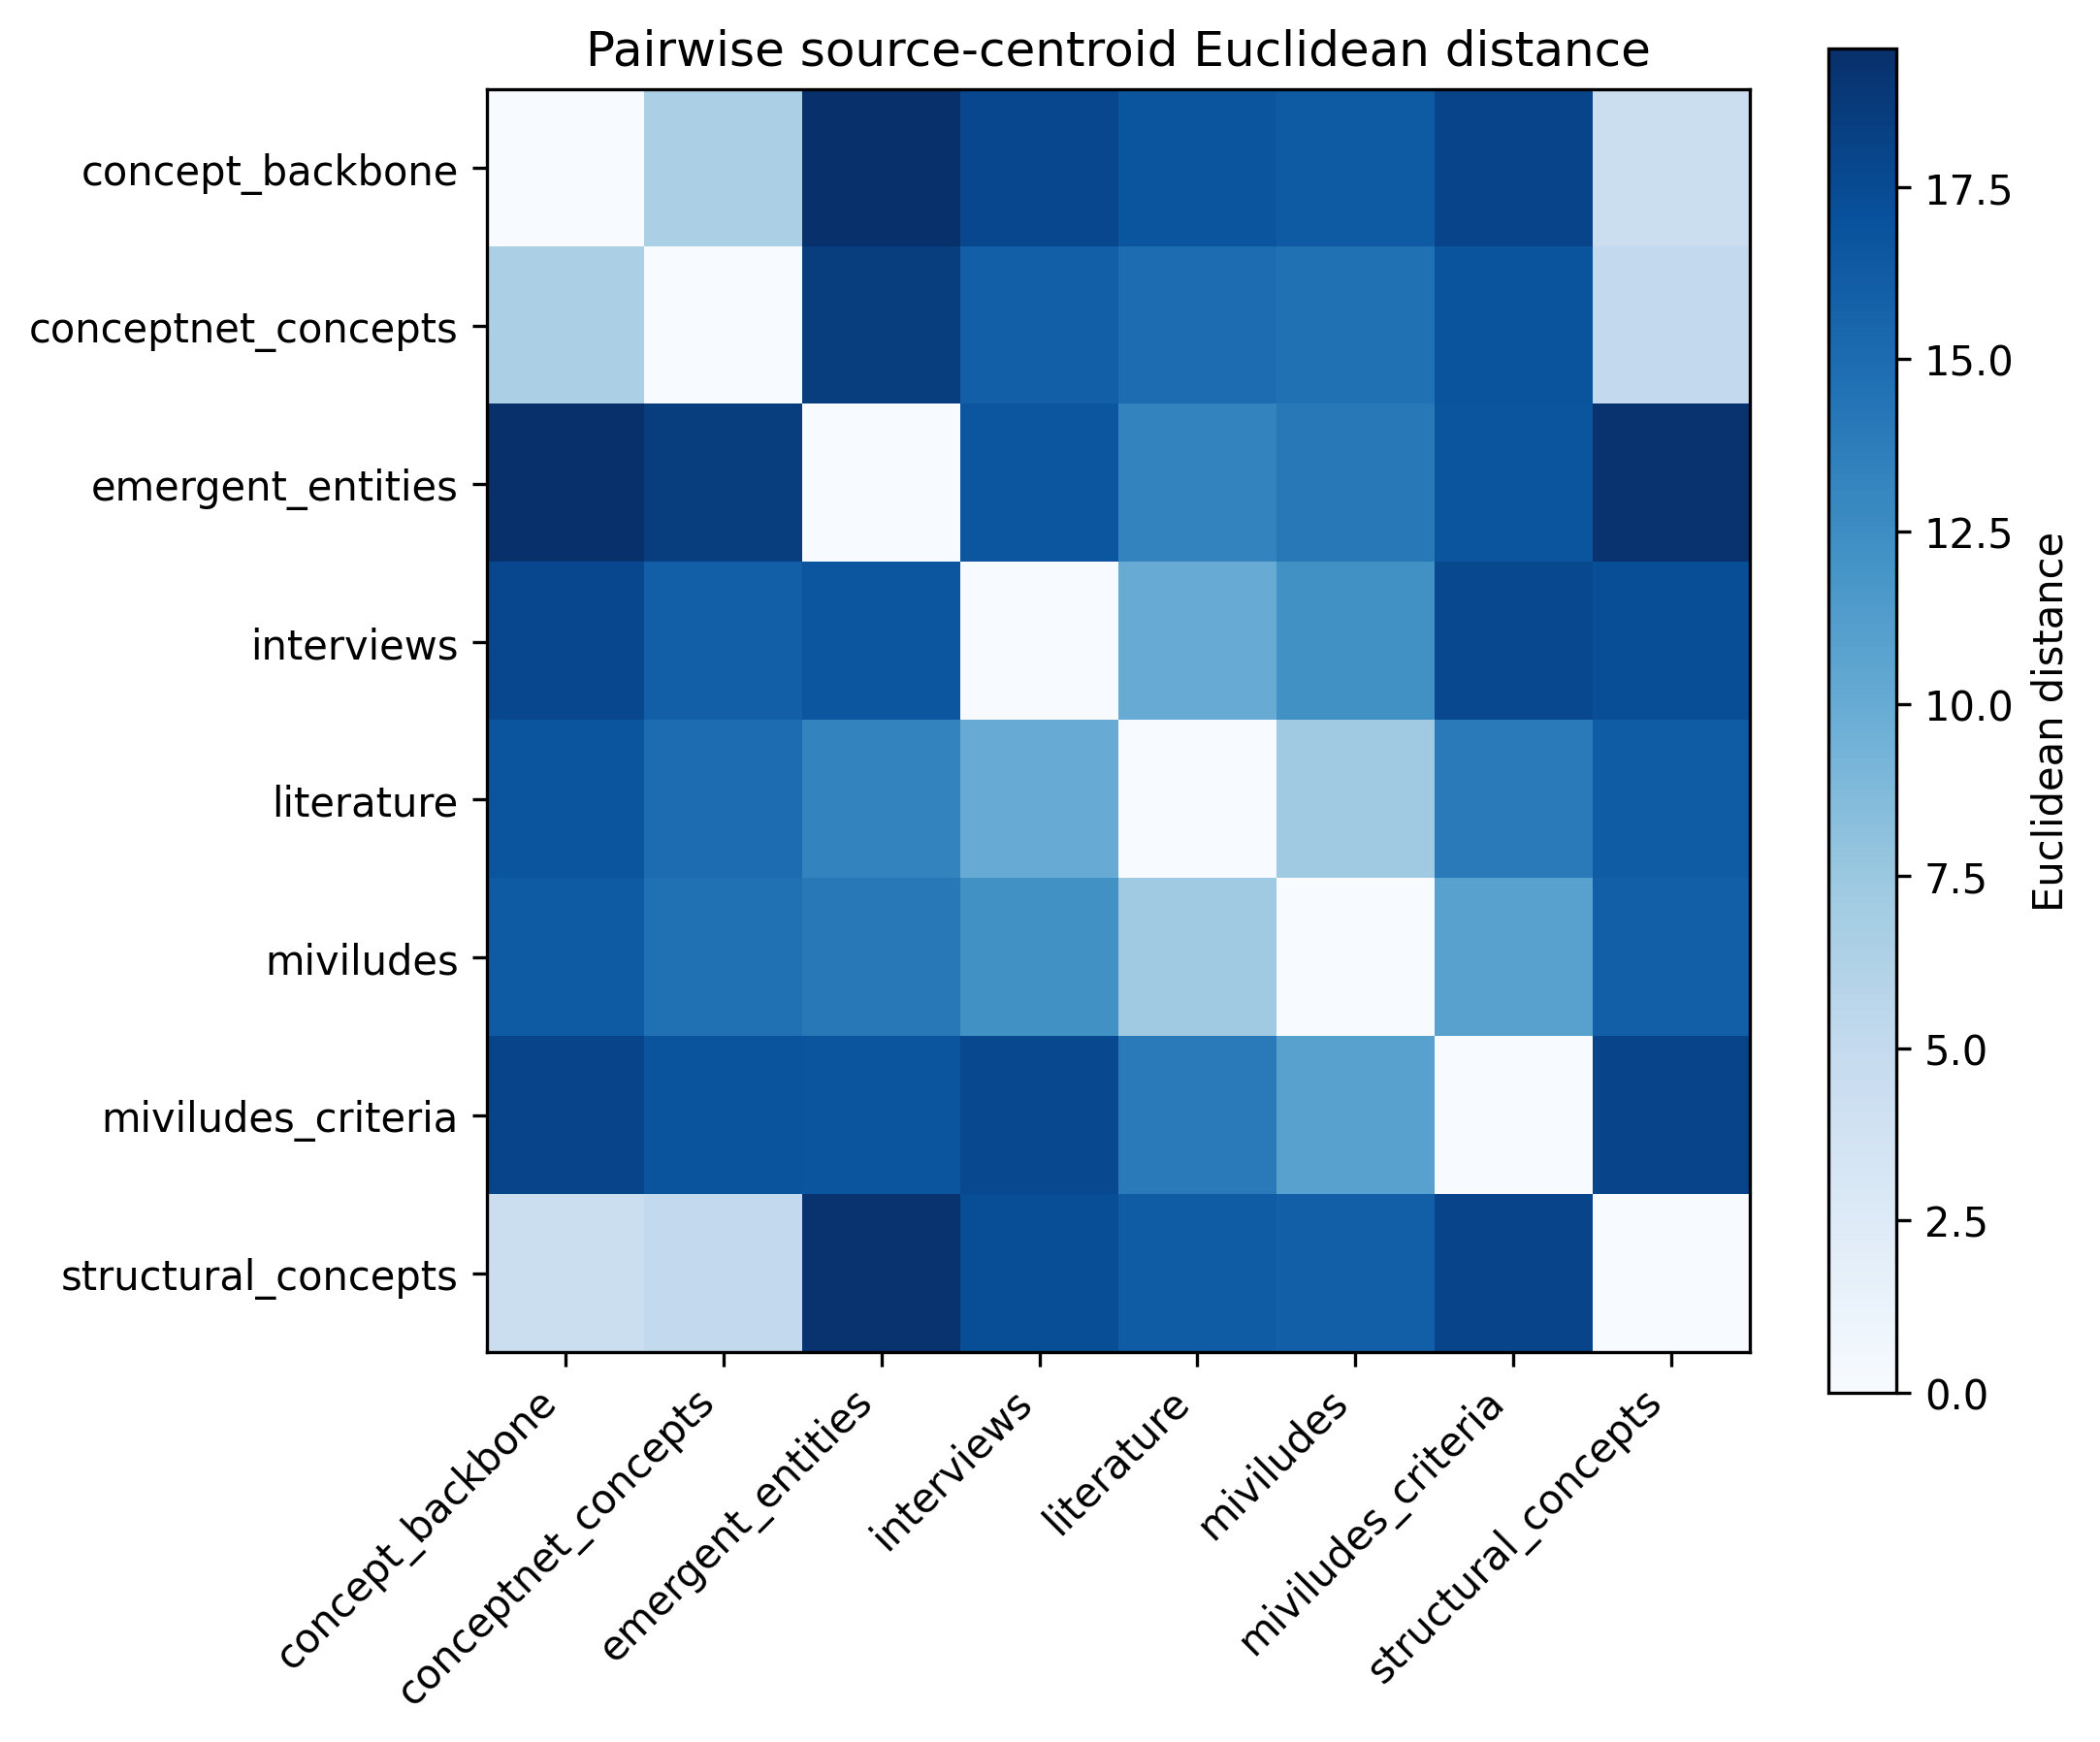
\includegraphics[width=0.85\textwidth]{figures/pairwise_source_centroid_heatmap.png}
\caption{Heatmap of pairwise centroid distances across all eight
sources. Darker/lighter cells indicate closer/further centroids;
see the module's own colour scale.}
\end{figure}

The same module also measured how far each of the three reference
vocabularies and the emergent-entities set sit from the combined
expression centroid (literature+MIVILUDES+interviews together, computed
three different ways -- see the CSV for the "full" vs.\
"reduced\_literature" vs.\ "equal\_weight" variants, which are never
merged into one number). Using the most direct ("full") variant:
concept\_backbone 16.70, structural\_concepts 16.18,
conceptnet\_concepts 14.92, emergent\_entities 13.20. The ordering is
consistent with how each vocabulary was built: emergent entities (drawn
directly from what the corpora mention) sit closest, the topic-neutral
concept backbone sits furthest, and the two vocabularies built as
deliberate middle grounds (structural concepts, ConceptNet-generalised
concepts) land in between -- with the ConceptNet-generalised set,
hand-picked for domain relevance, closer than the corpus-mined but
unreviewed structural-concepts list. This is a centroid-level comparison
only (not adjusted for the three vocabularies' very different sizes --
3,000/1,500/195 terms); a separate, size-controlled comparison exists
alongside it for exactly that reason and is not to be averaged with this
one.

\subsection{Cluster structure: do the three sources actually separate?}
\label{sec:cluster}
\jargon{Module: \texttt{analyze\_cluster\_structure}}

Centroid distances (previous section) say how far apart the
\emph{average} positions are, but not whether the sources form genuinely
separate regions or heavily overlapping clouds. This module answers that
with k-nearest-neighbour composition and a silhouette score, using an
\jargon{equal-$n$} sampling scheme (each of the three sources
down-sampled to the same count before comparing, since literature so
outnumbers the other two that an uncontrolled comparison would just be
dominated by it) and bootstrap-resampled 100 times for a confidence
interval.

\begin{table}[h!]
\centering
\small
\begin{tabular}{lllrrr}
\toprule
$k$ & Query source & Neighbour source & Mean fraction & 95\% CI \\
\midrule
10 & literature & literature  & 0.316 & [0.283, 0.350] \\
10 & literature & miviludes   & 0.307 & [0.273, 0.338] \\
10 & literature & interviews  & 0.378 & [0.347, 0.413] \\
10 & miviludes  & literature  & 0.112 & [0.089, 0.137] \\
10 & miviludes  & miviludes   & 0.674 & [0.641, 0.720] \\
10 & miviludes  & interviews  & 0.213 & [0.183, 0.241] \\
10 & interviews & literature  & 0.057 & [0.043, 0.074] \\
10 & interviews & miviludes   & 0.088 & [0.072, 0.104] \\
10 & interviews & interviews  & 0.855 & [0.837, 0.875] \\
\bottomrule
\end{tabular}
\caption{k-NN neighbour composition (equal-$n$, $k=10$): of a query
point's 10 nearest neighbours, what fraction come from each source, on
average. Rows sum to 1 within each query source.}
\end{table}

Reading this table in plain terms: interview points are the most
"self-clustering" of the three -- 85.5\% of an interview point's nearest
neighbours are other interview points. MIVILUDES points are also fairly
self-clustering (67.4\%). Literature is the least self-clustering of the
three: only 31.6\% of a literature point's nearest neighbours are other
literature points, with the rest split fairly evenly toward MIVILUDES
(30.7\%) and interviews (37.8\%) -- meaning literature, despite being
the largest and most "central" source in raw point count, does not
occupy a tightly separate region; it sits closer to a shared middle
ground than either MIVILUDES or the interviews do relative to it. The
$k=20$ results (in the same CSV) show the same pattern.

\begin{figure}[h!]
\centering
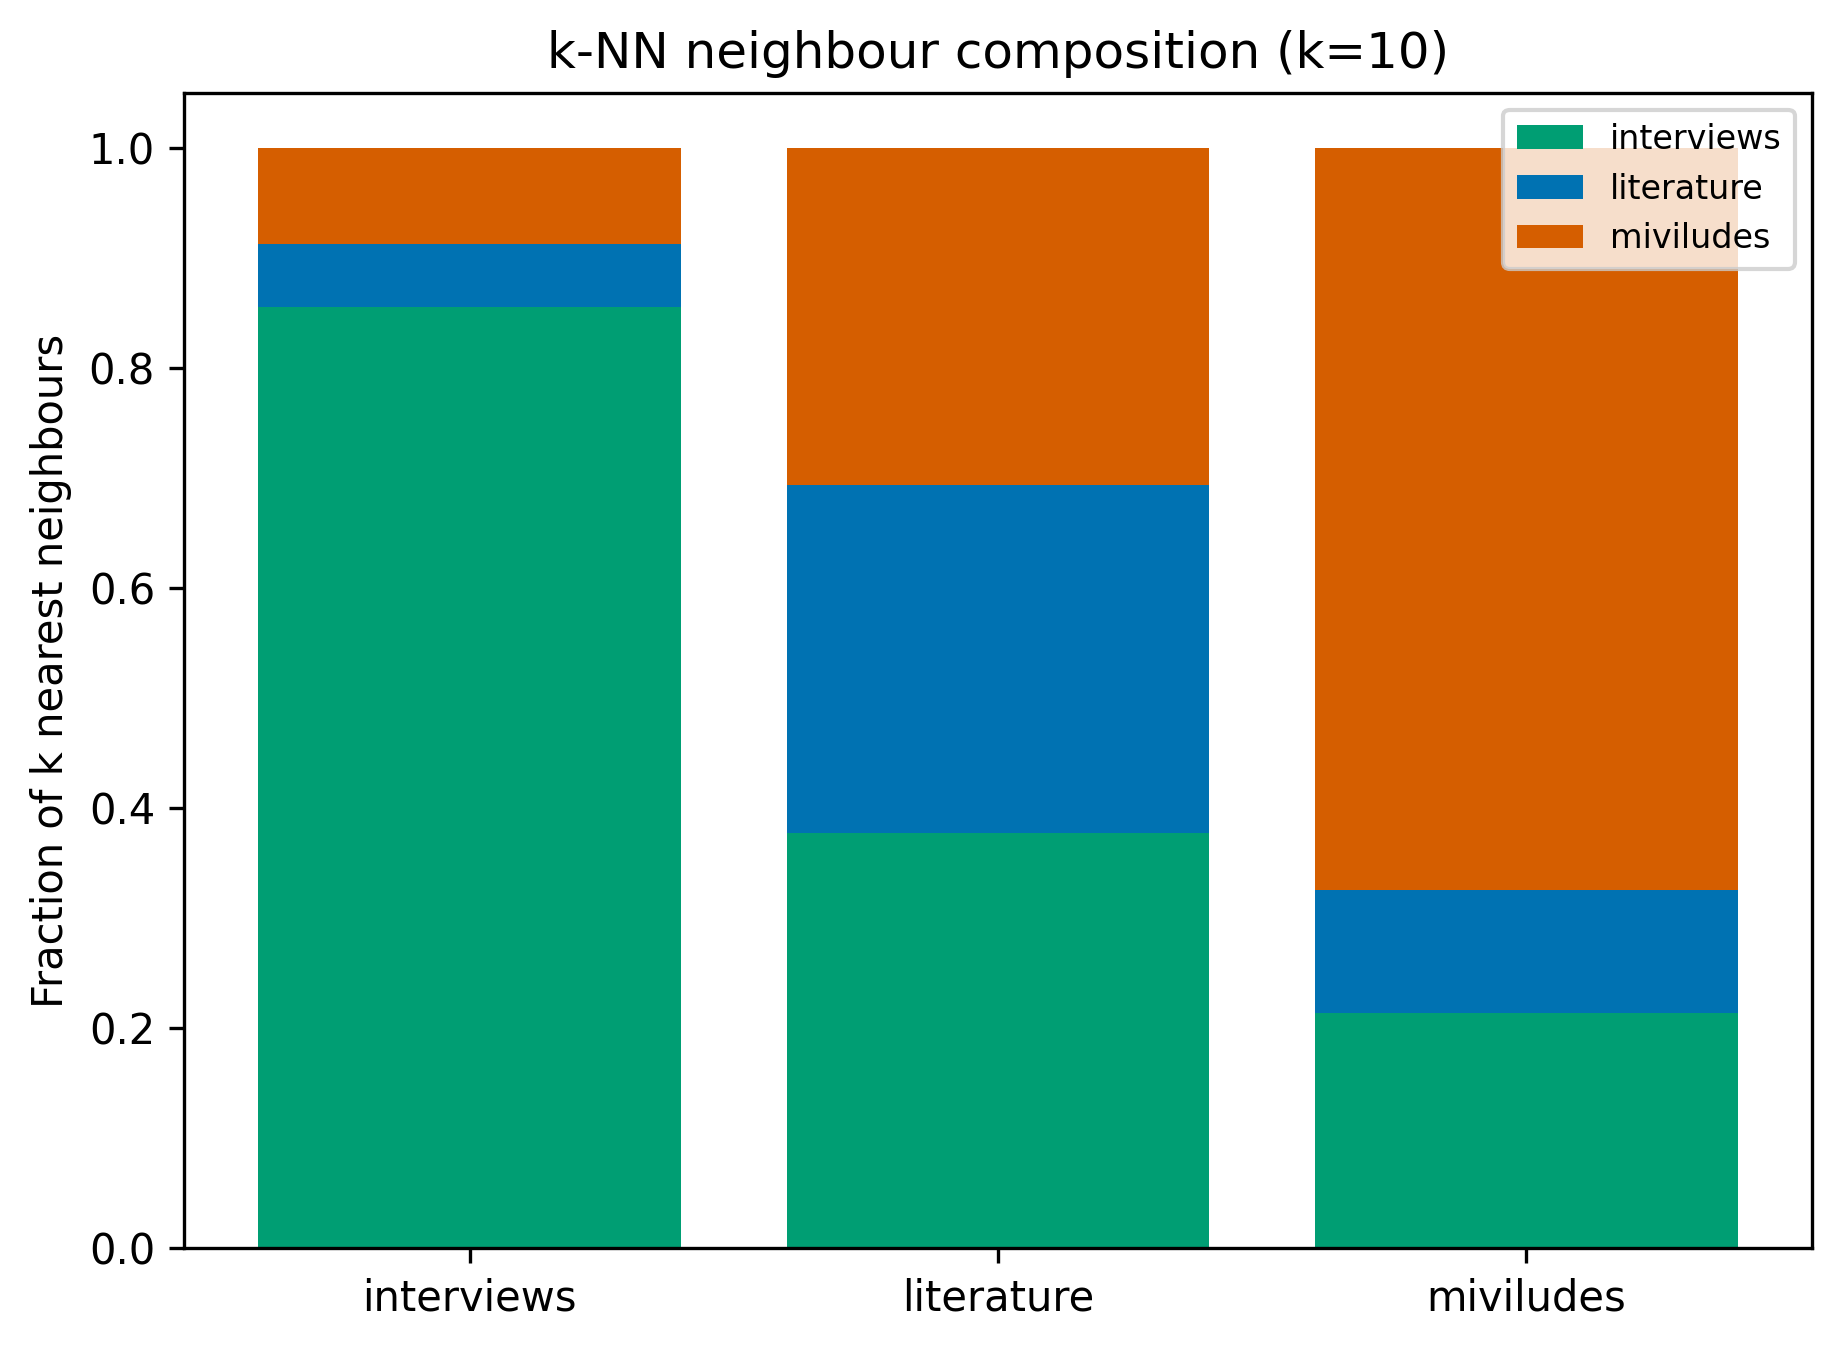
\includegraphics[width=0.85\textwidth]{figures/knn_composition_equal_n_k10.png}
\caption{k-NN neighbour composition at $k=10$, equal-$n$ sampling,
visualised.}
\end{figure}

The silhouette score for the three-source grouping, same equal-$n$
sampling, is \textbf{0.019} (95\% CI [0.017, 0.022]) -- very close to
zero. In plain terms: treating "literature / MIVILUDES / interviews" as
three geometric clusters does not match the actual shape of the data
well at all. The three sources overlap substantially rather than
forming three separate blobs -- consistent with, though not the same
measurement as, the mixed k-NN composition above.

\begin{figure}[h!]
\centering
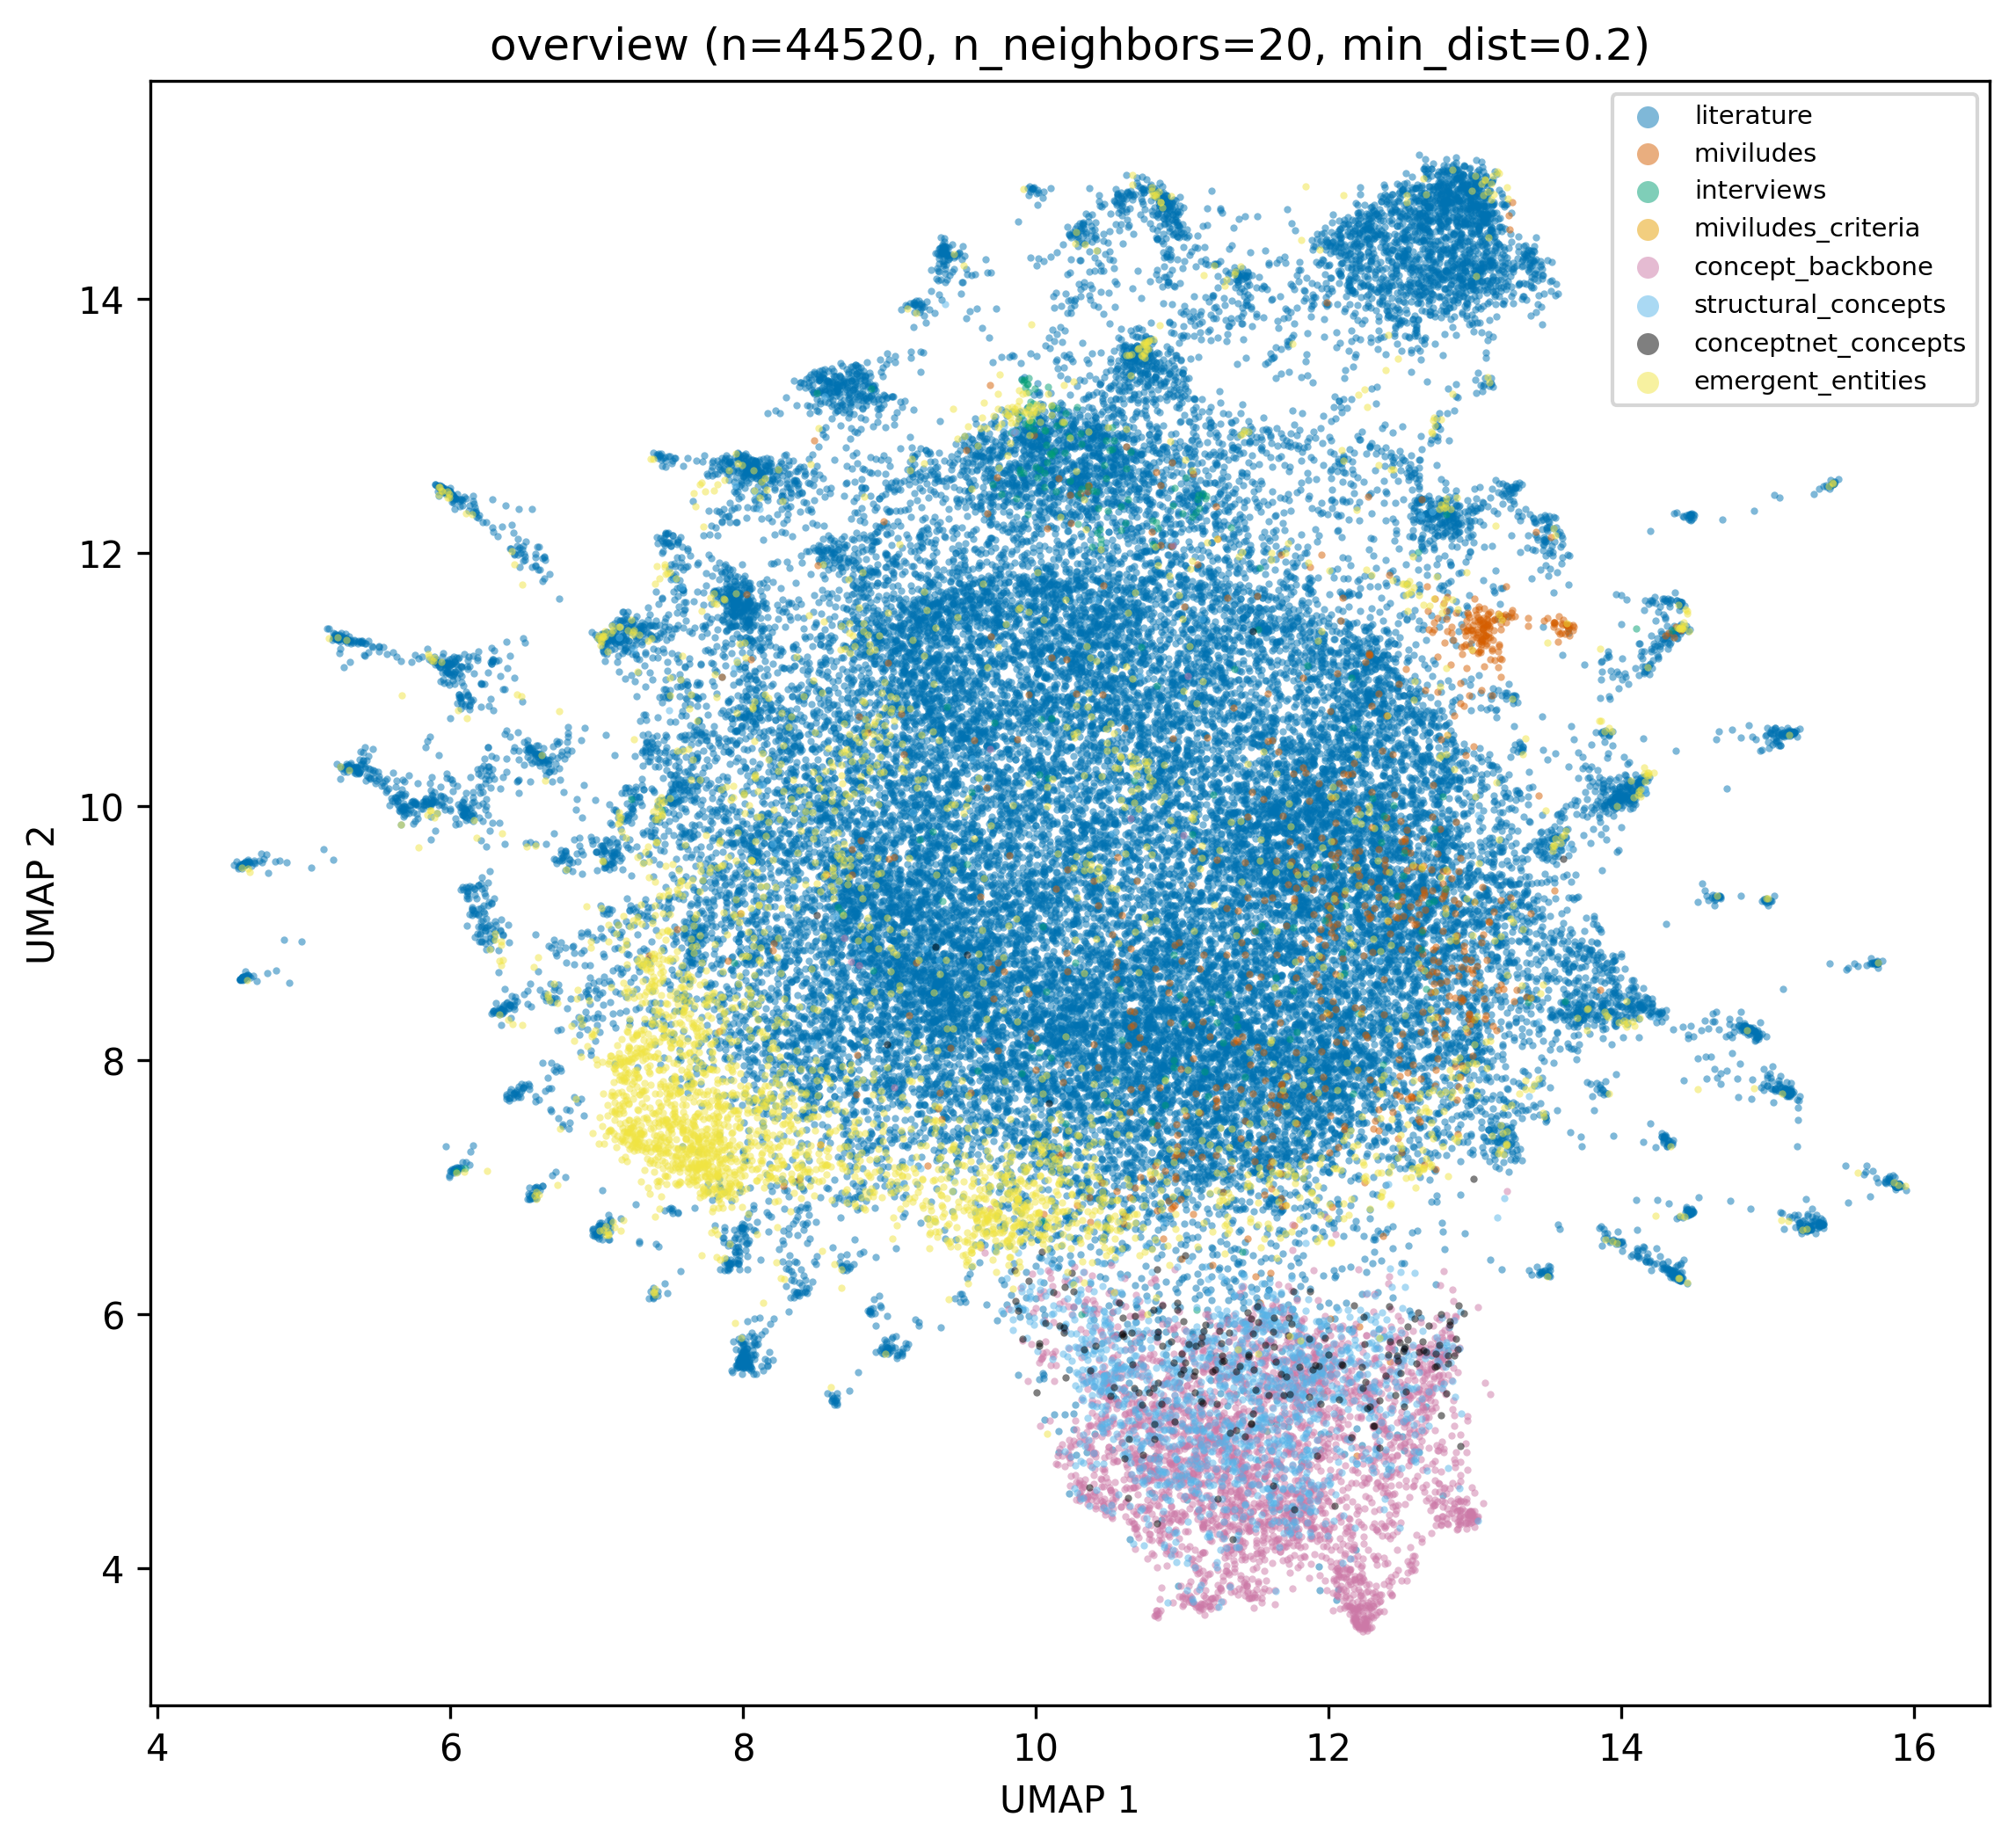
\includegraphics[width=0.85\textwidth]{figures/umap_overview_by_source_dataset_n20_d0.2.png}
\caption{Whole-space UMAP overview, coloured by source dataset. At over
44{,}000 points this is a dense, exploratory picture -- useful for a
general sense of overlap and shape, not for reading off any one specific
comparison.}
\end{figure}

\begin{figure}[h!]
\centering
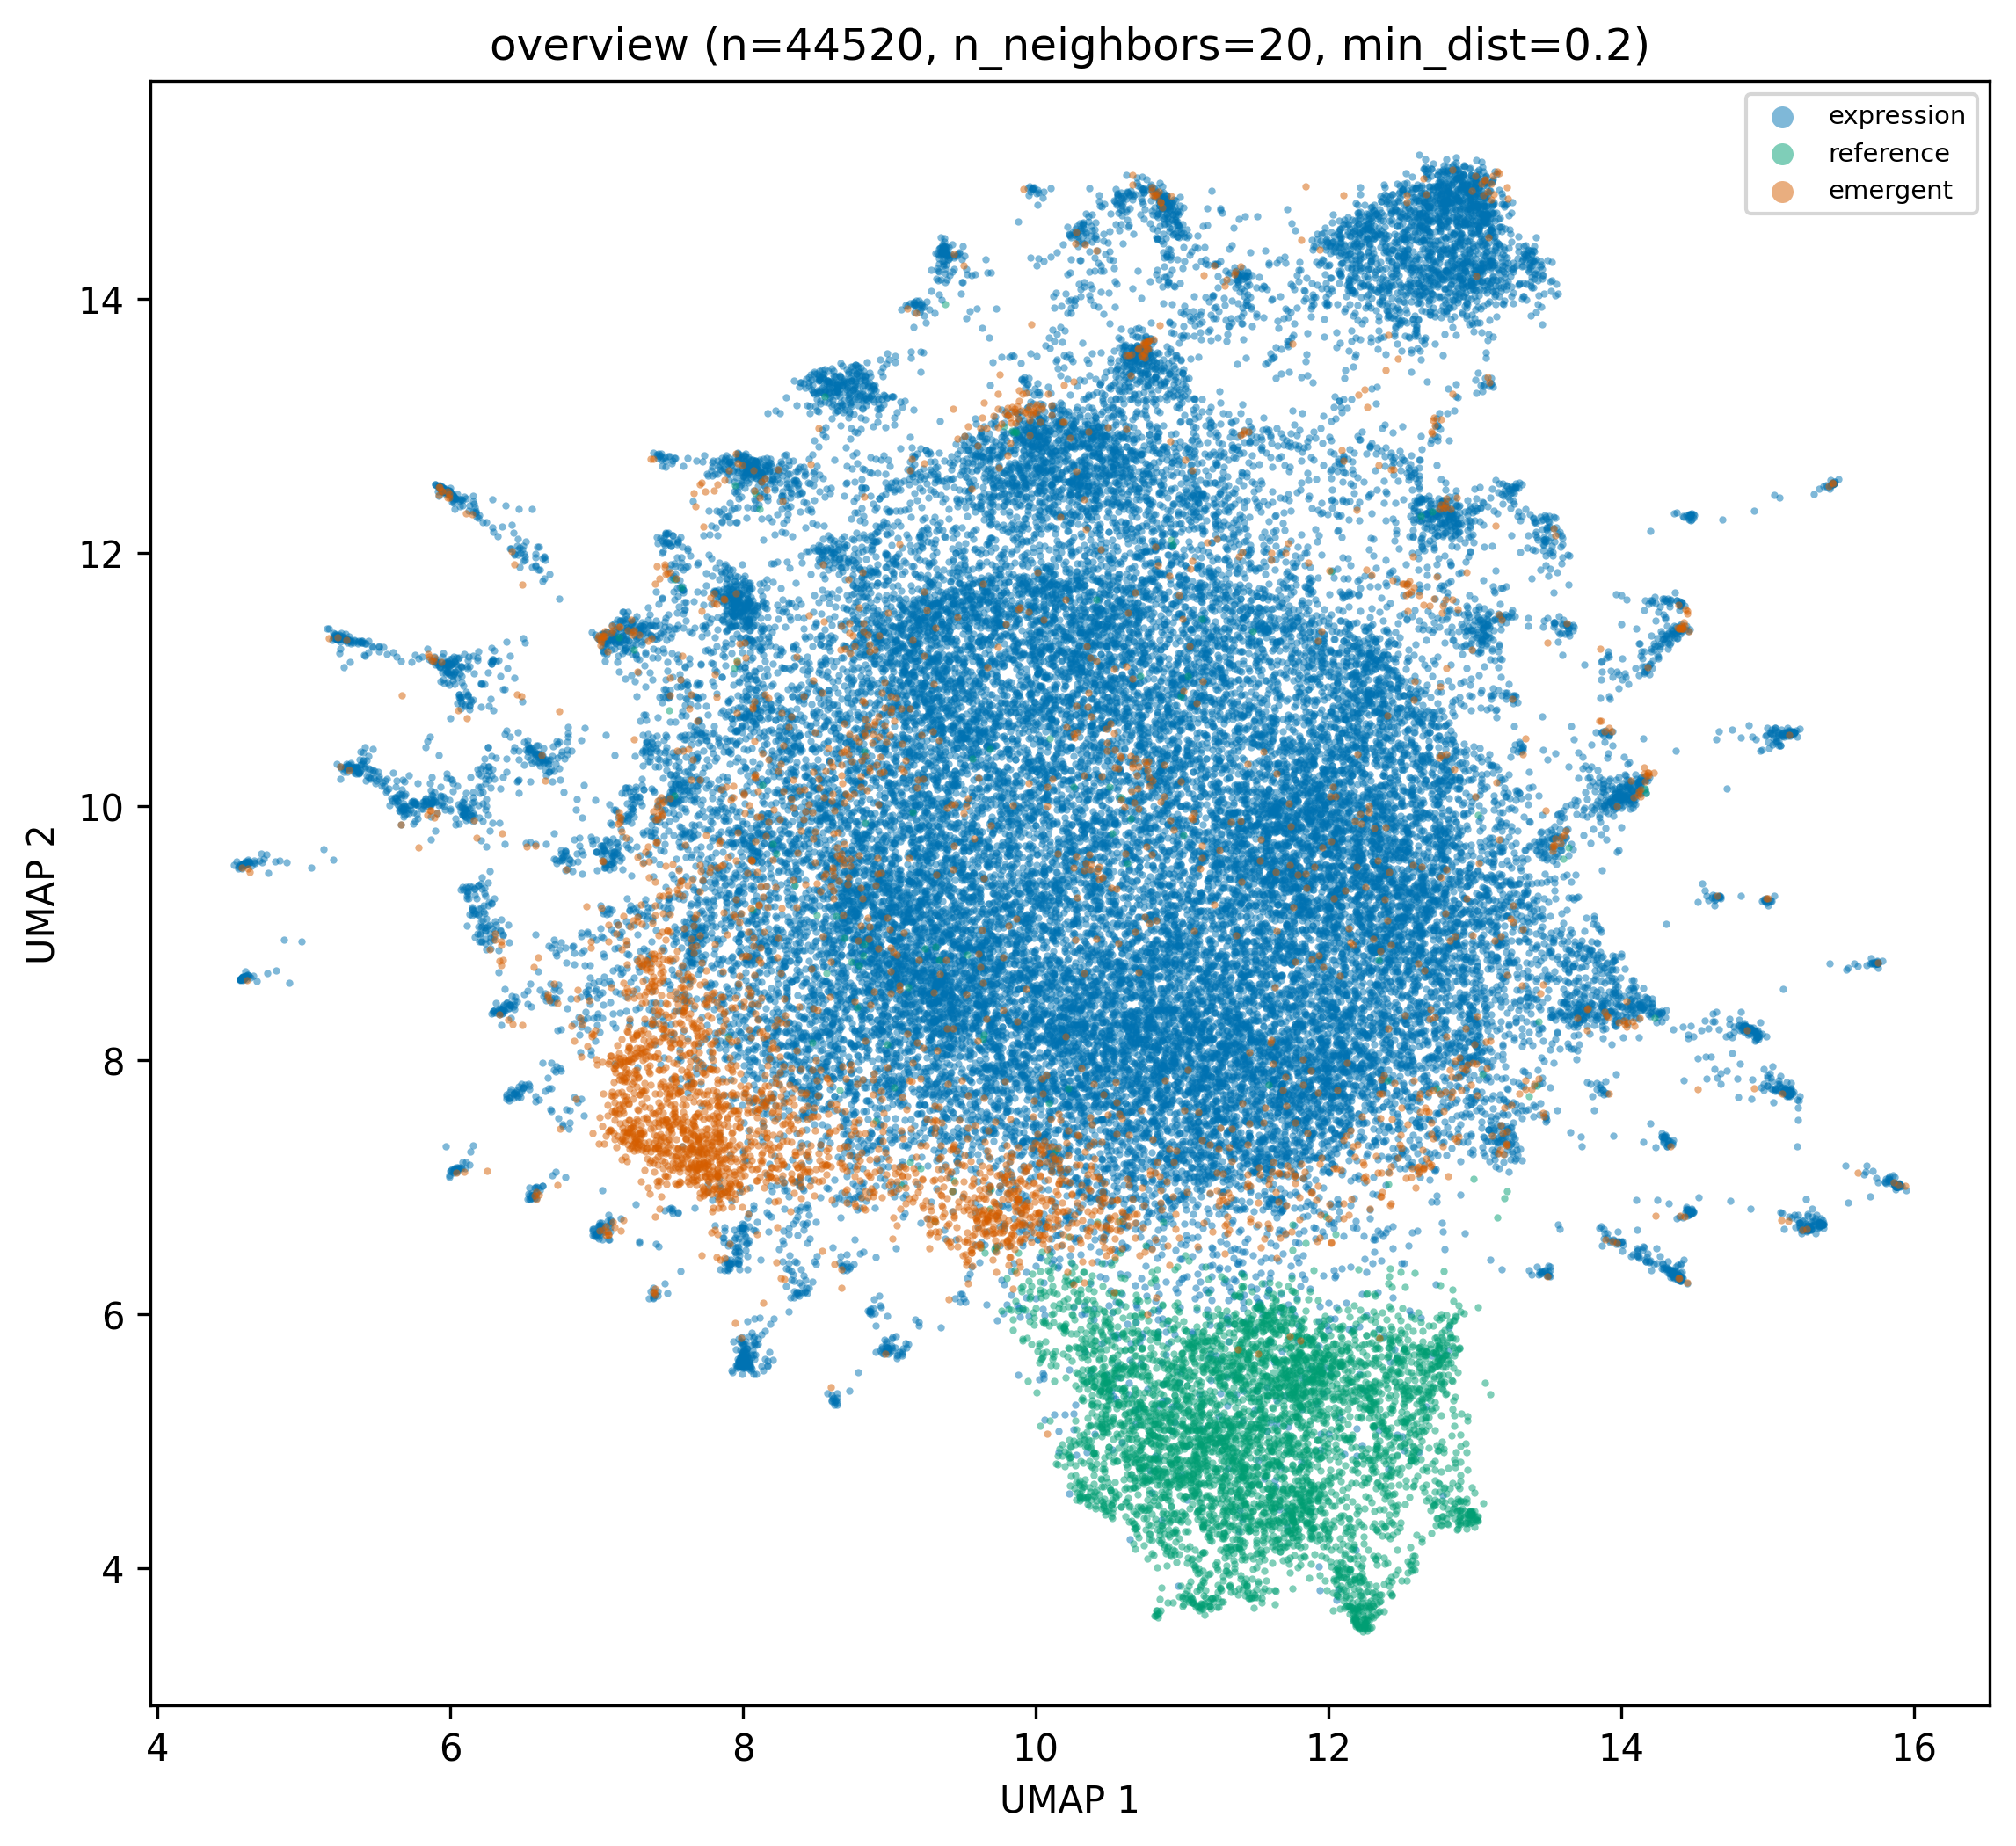
\includegraphics[width=0.85\textwidth]{figures/umap_overview_by_point_role_n20_d0.2.png}
\caption{The same whole-space UMAP layout, coloured by point role
(expression / reference / emergent) instead of source dataset.}
\end{figure}

\subsection{Criterion neighbours: what sits near MIVILUDES's 17 official criteria?}
\jargon{Module: \texttt{analyze\_criterion\_neighbours}}

For each of MIVILUDES's 17 official criteria (e.g.\ "authoritarian,
opaque group," "deceptive recruitment," "difficulty leaving the group"),
this module finds which literature, MIVILUDES, and interview expressions
sit closest to it in the shared space, and which of the three reference
vocabularies' terms are nearest.

Because MIVILUDES's criteria are officially in French but the rest of
the corpus is mostly English, this comparison is run in \textbf{three
separate, never-merged ways}: (1) the criteria in their original French,
projected into the main shared space (the primary representation); (2)
the criteria's own stored English translations, projected through the
exact same fitted transform into the identical space (the main
cross-check on whether language affects the result); and (3) a simpler,
secondary diagnostic comparing raw English embeddings by cosine
similarity, without any of the shared-space machinery (not directly
comparable in scale to the other two).

\begin{plainbox}[Language sensitivity result]
Comparing which corpus is "nearest" to each of the 17 criteria under the
French-original versus English-translation representations: \textbf{0
out of 17} criteria change which corpus is nearest. Comparing against
the simpler raw-cosine diagnostic: \textbf{1 out of 17} criteria differ.
In plain terms: the choice of French vs.\ English representation, within
the main shared space, essentially does not change which corpus each
criterion is closest to.
\end{plainbox}

\begin{figure}[h!]
\centering
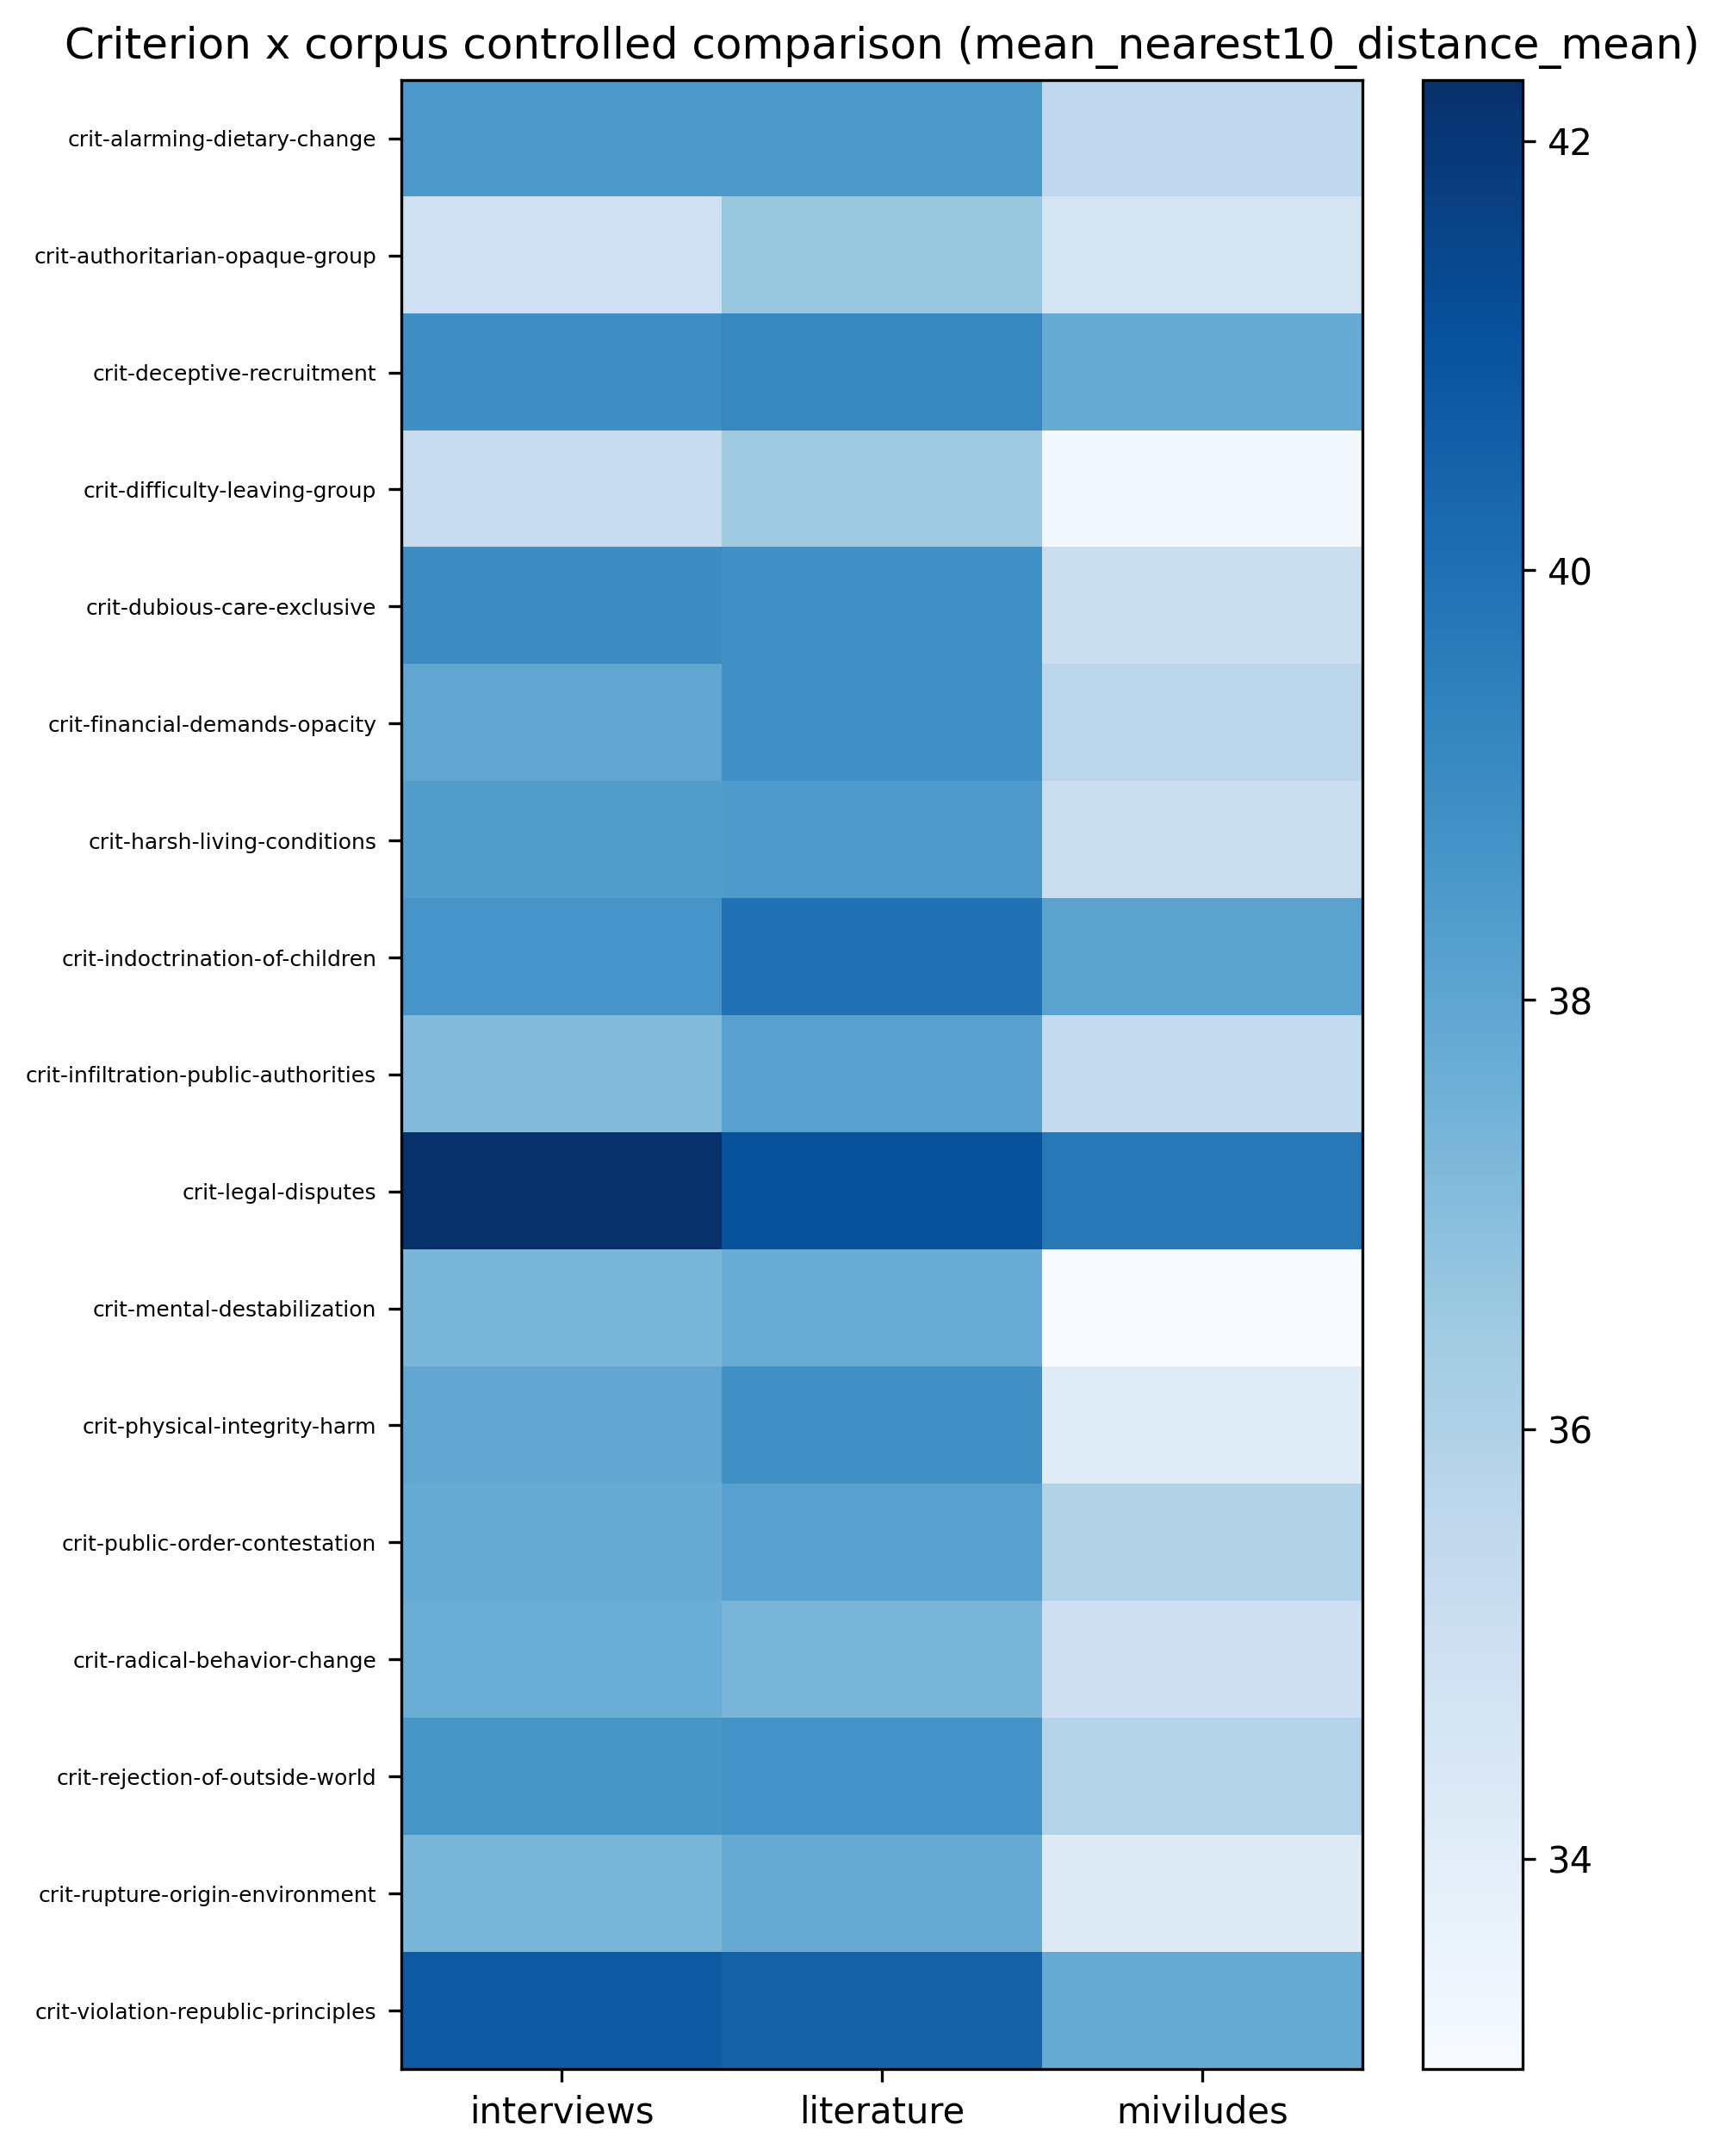
\includegraphics[width=0.85\textwidth]{figures/criterion_corpus_heatmap.png}
\caption{Heatmap of each of the 17 MIVILUDES criteria against the three
expression corpora (French-primary shared-space representation).}
\end{figure}

A focused, readable 2-D projection is also generated per criterion,
showing just that criterion and its nearest neighbours rather than the
whole 44,000-point space. As one example:

\begin{figure}[h!]
\centering
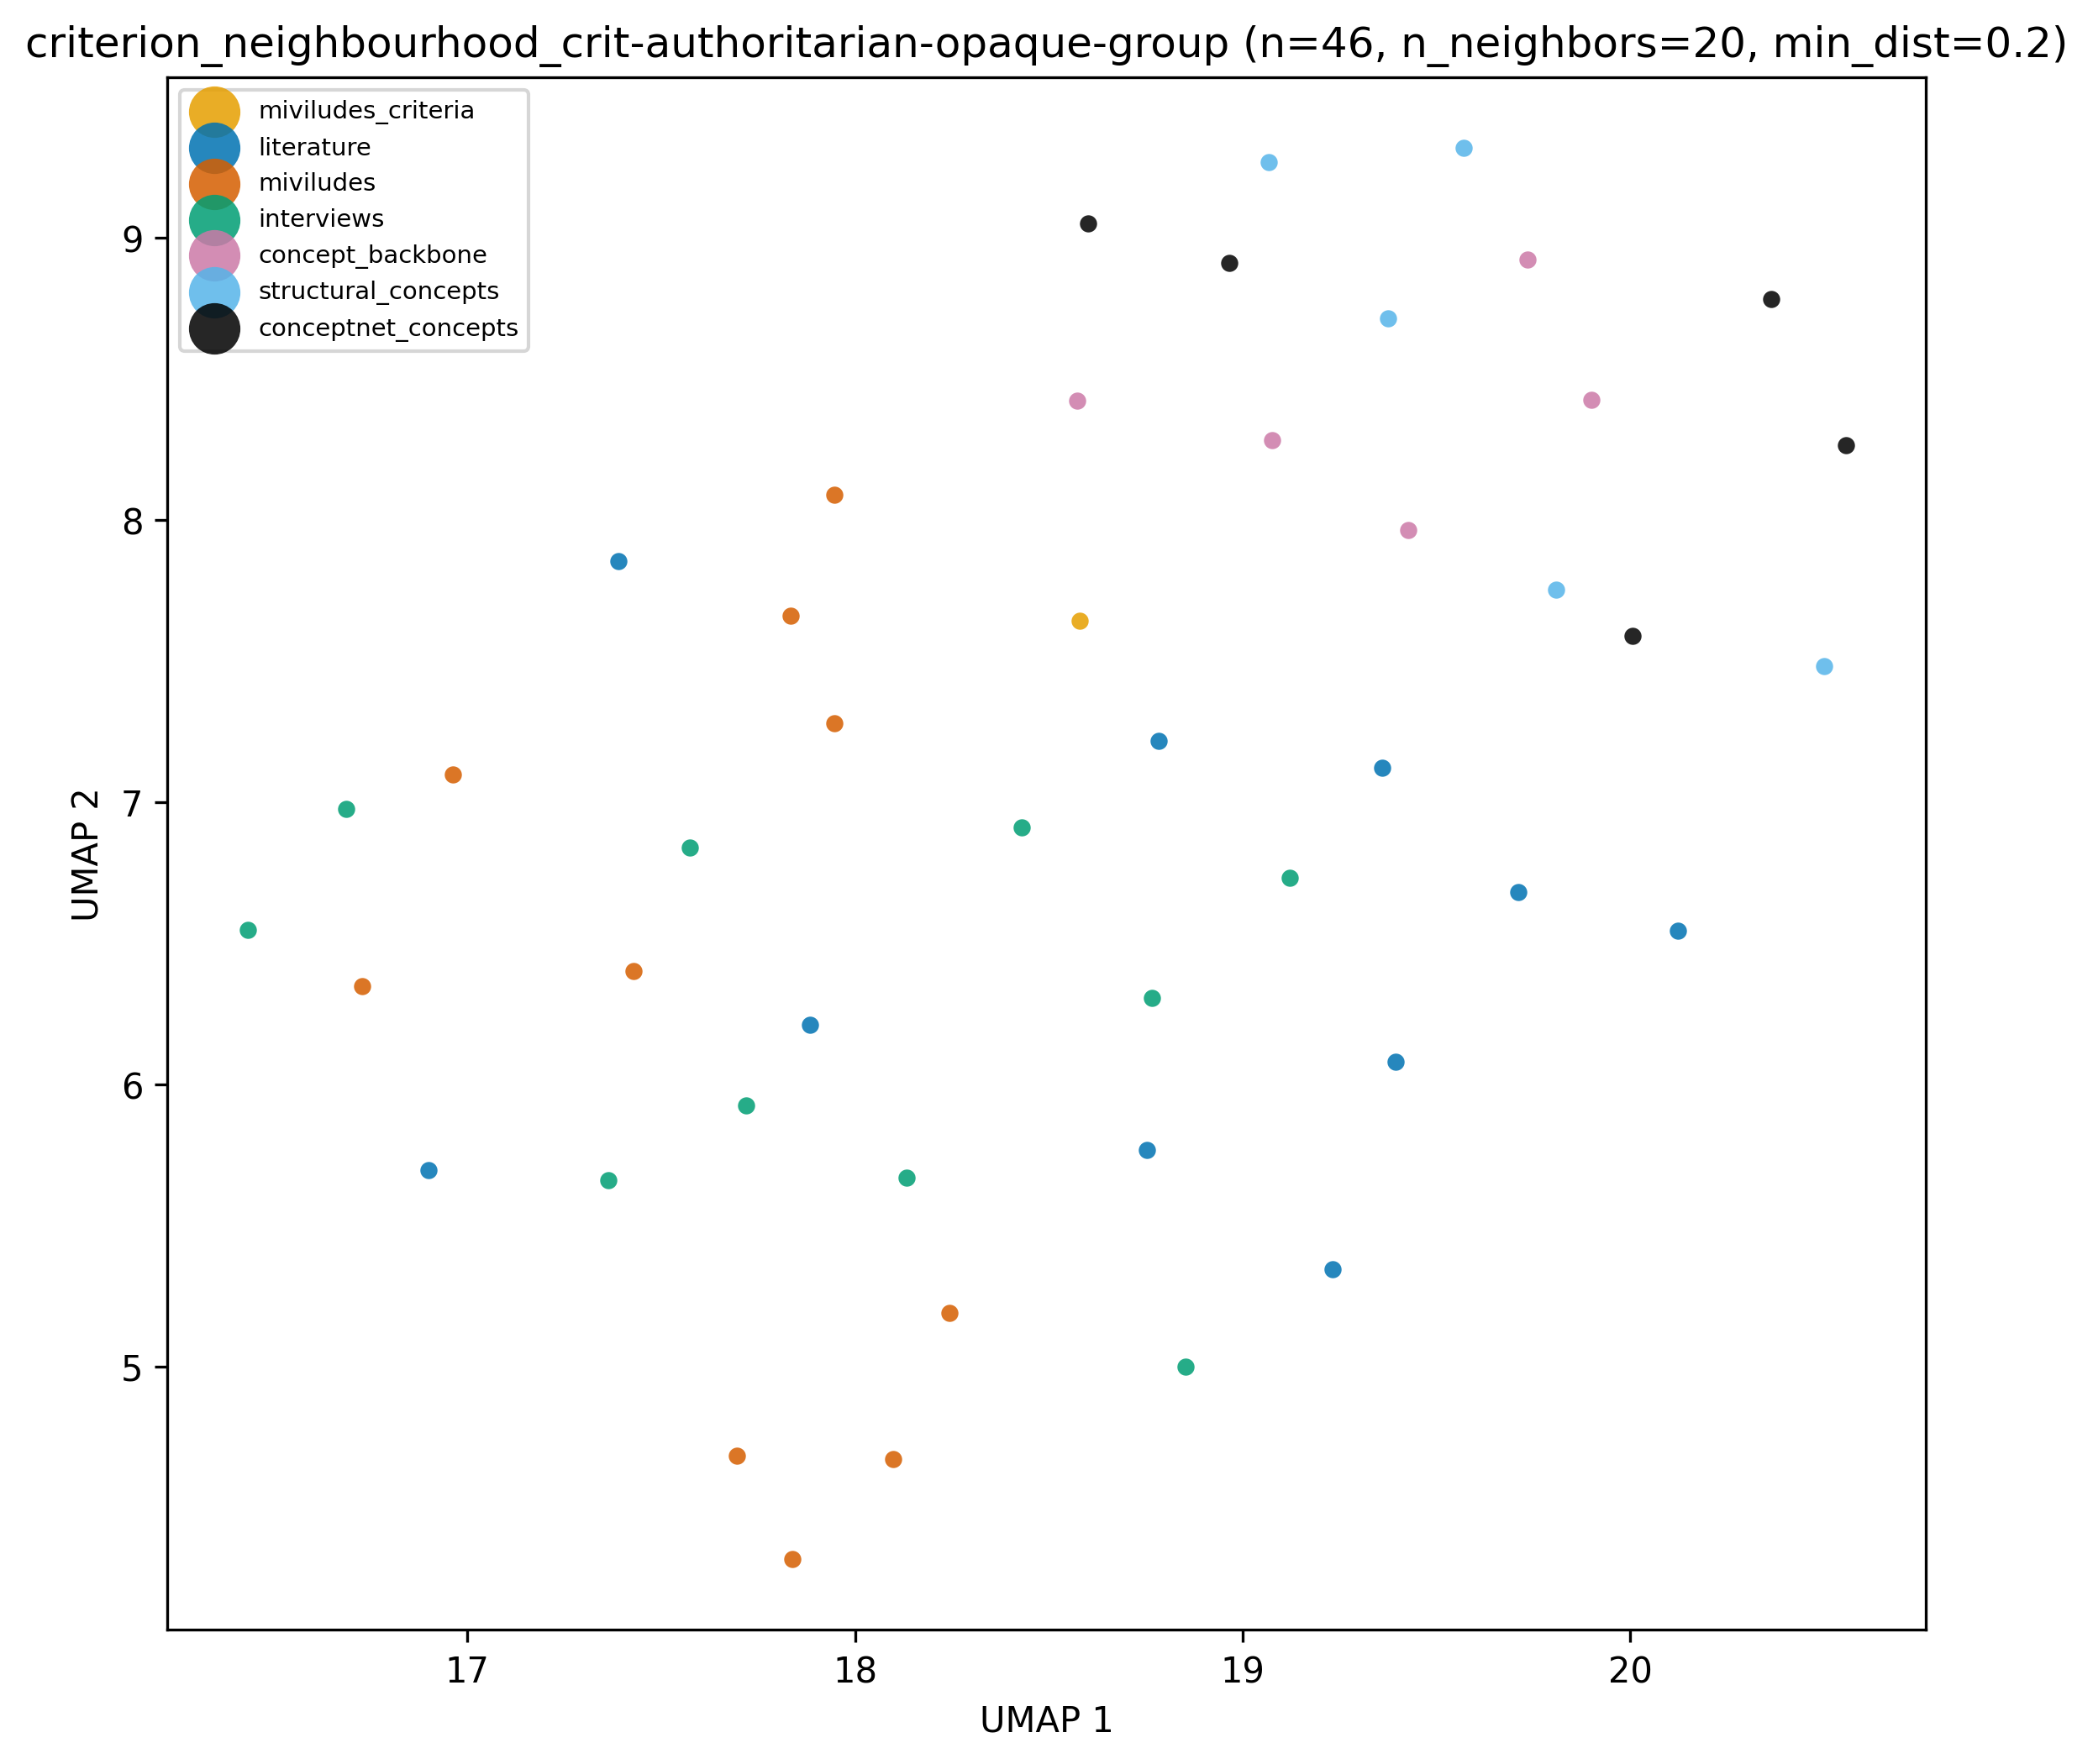
\includegraphics[width=0.8\textwidth]{figures/umap_criterion_neighbourhood_crit-authoritarian-opaque-group_by_source_dataset_n20_d0.2.png}
\caption{Focused UMAP neighbourhood around the "authoritarian, opaque
group" criterion, coloured by source dataset. One of 17 such
per-criterion figures generated this run; the rest are in the run's own
\texttt{generate\_figures/} directory.}
\end{figure}

\subsection{Interview initial exemplars: what do people say first?}
\label{sec:exemplars}
\jargon{Module: \texttt{analyze\_initial\_exemplars}}

This is where the manually-reviewed interview-prototype layer
(Stage~6, Section~\ref{sec:jargon}'s point-role discussion) is actually
used. For each of the 26 interviews, the participant's verified first
response to the opening prompt was placed in the shared space and its
distance measured to: each of the 17 MIVILUDES criteria, each reference
vocabulary, each expression-corpus centroid, and the nearest literature
/ MIVILUDES / other-interview expressions.

Each response was also given a descriptive code, \texttt{exemplar\_type}
-- not a claim about a natural category, just a label for what kind of
answer it was (e.g.\ a named group, a "classic" religious-NRM
description, a digital/technology reference, something metaphorical, or
simply unclear).

\begin{table}[h!]
\centering
\small
\begin{tabular}{lr}
\toprule
Exemplar type & Count \\
\midrule
unclear & 11 \\
classic\_nrm\_or\_religious\_group & 4 \\
named\_group\_or\_movement & 3 \\
metaphorical\_or\_other & 2 \\
mixed & 2 \\
digital\_or\_technology & 1 \\
organisation\_or\_institution & 1 \\
unavailable (no qualifying claim in transcript) & 1 \\
\bottomrule
\end{tabular}
\caption{Distribution of the 26 interviews' opening responses by
descriptive type. "Unclear" (11/26) is the largest single group --
these are responses that describe a feeling or a vague scenario rather
than naming a specific group or a textbook definition (e.g.\
"Something suspicious, something dangerous, something not normal").}
\end{table}

\begin{figure}[h!]
\centering
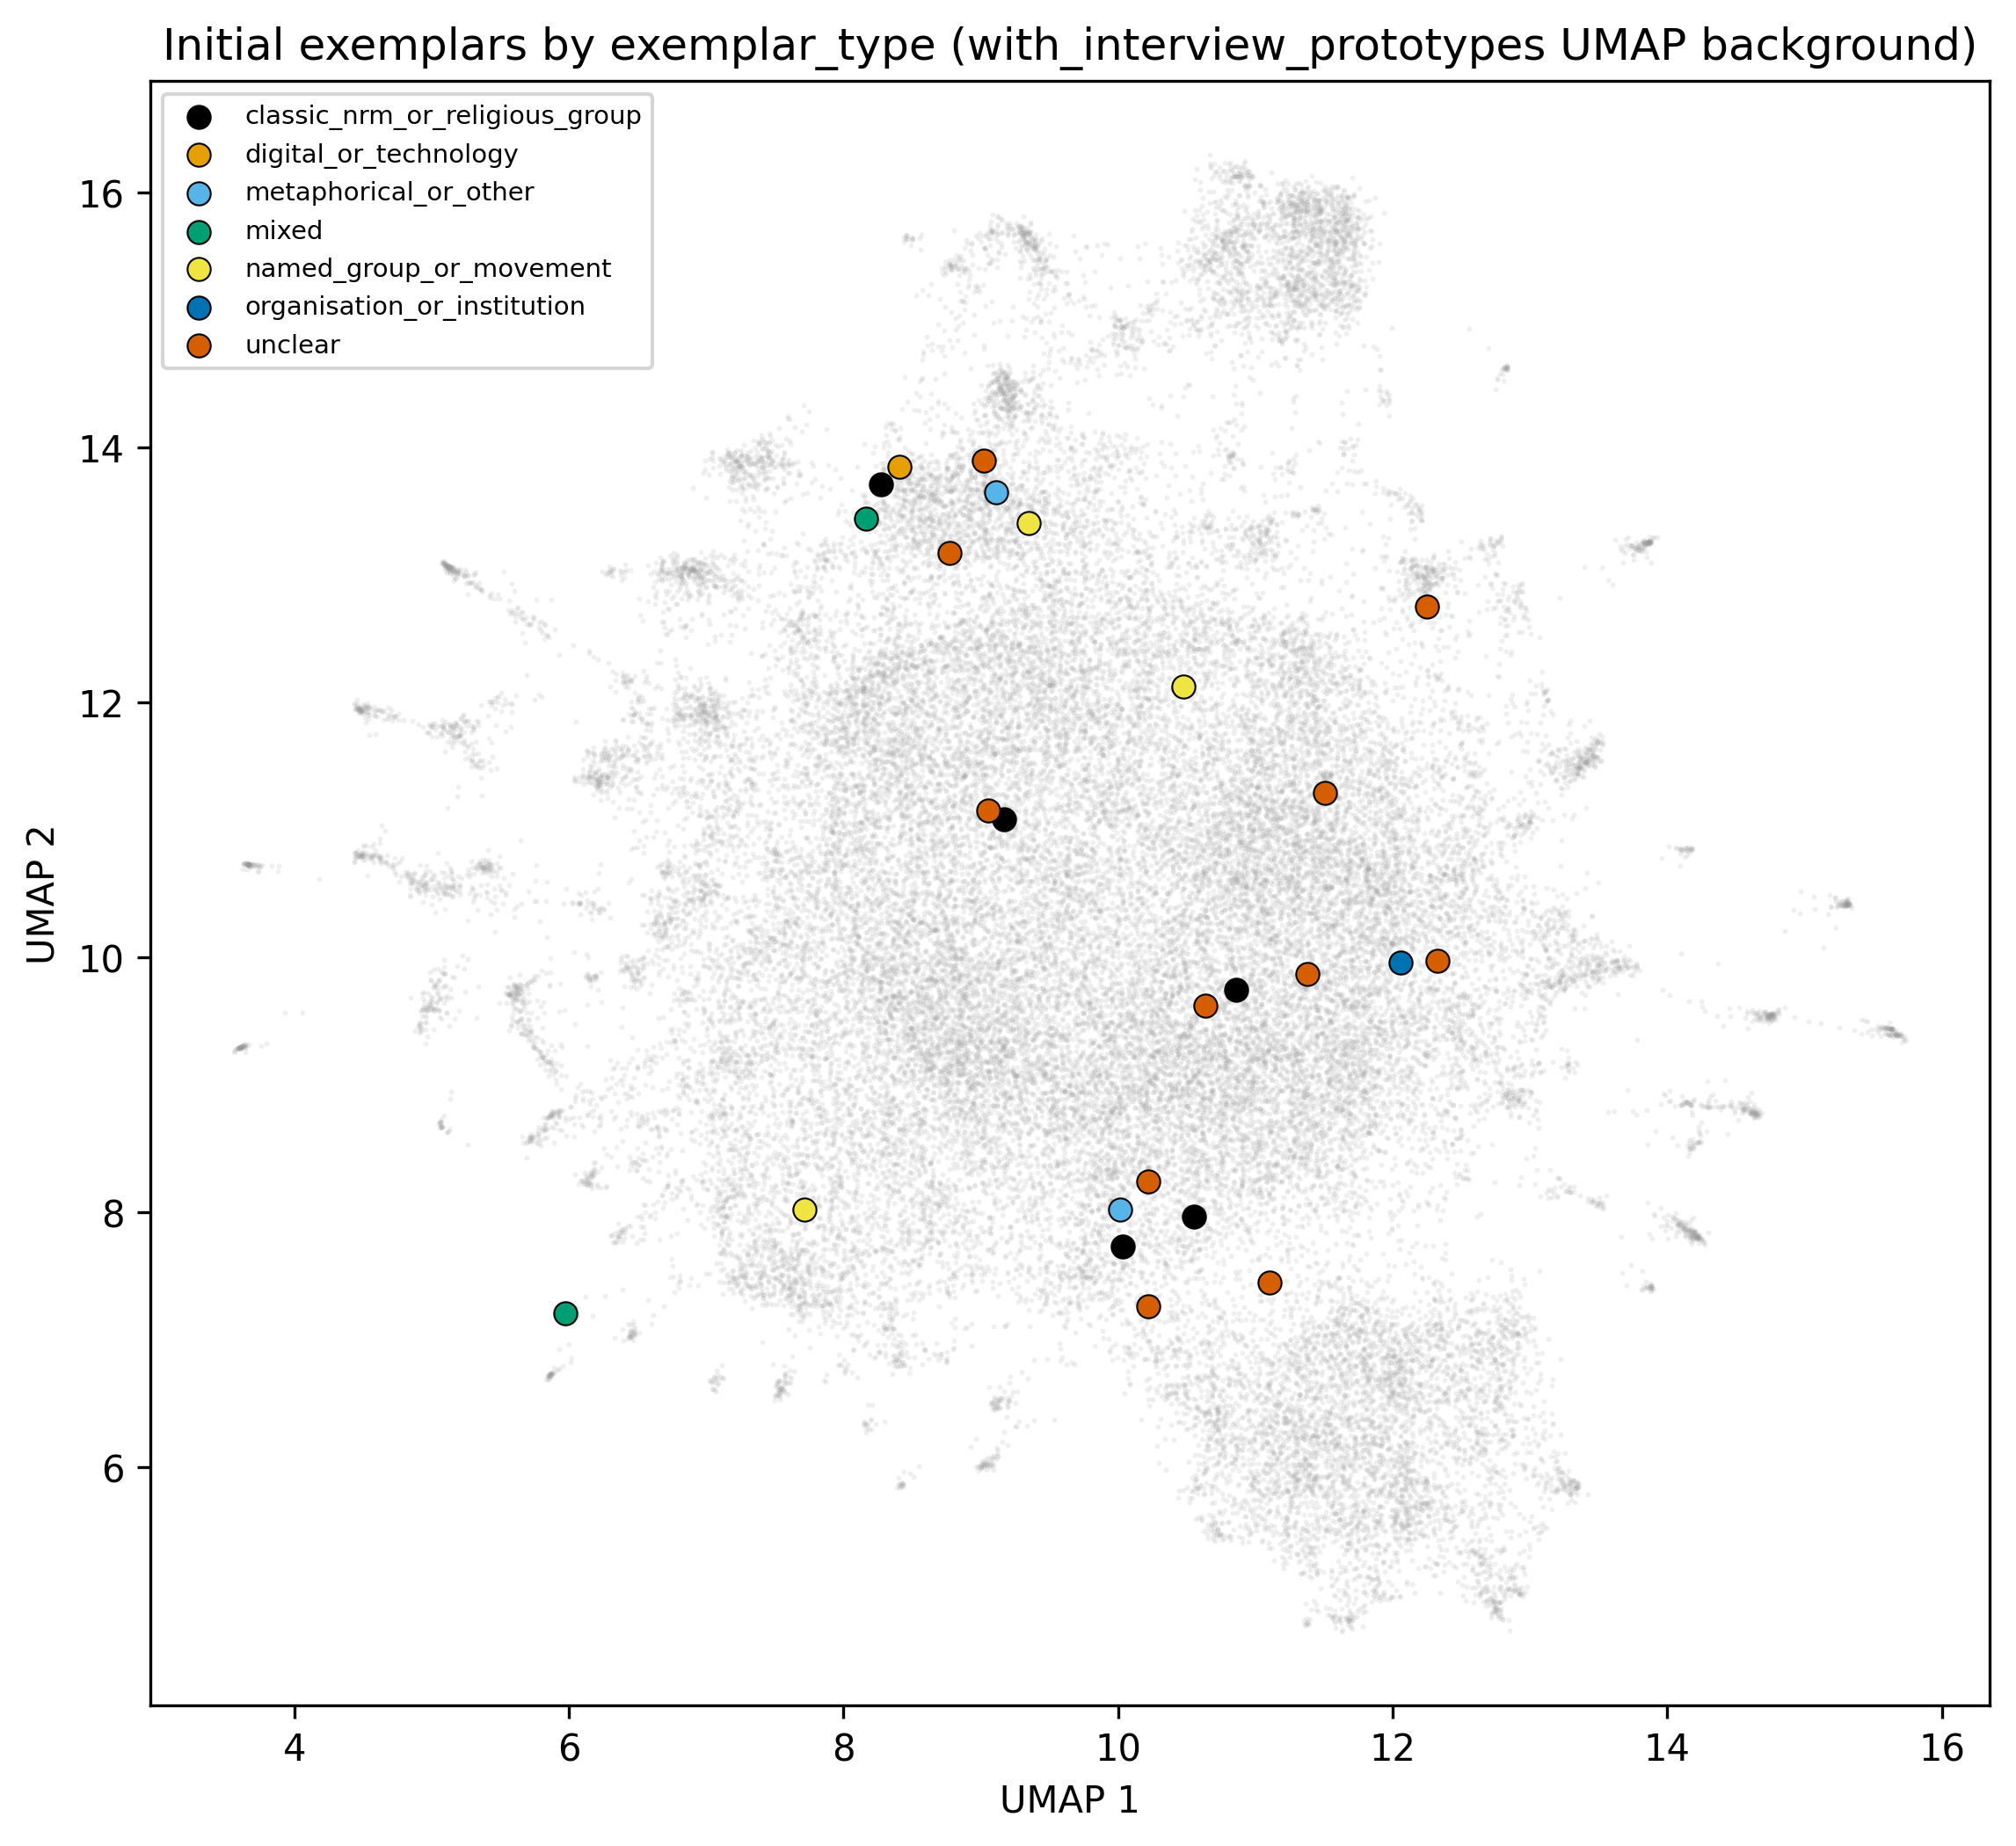
\includegraphics[width=0.75\textwidth]{figures/initial_exemplars_by_type.png}
\caption{Interview opening responses grouped by exemplar type.}
\end{figure}

Concretely, the 26 opening responses ranged from named groups ("Ku Klux
Klan," "Illuminati," "Charles Manson -- and CIA") through classic
religious-NRM descriptions ("smaller church denominations with a
charismatic leader and their own little special lore") to
metaphorical/other uses entirely disconnected from the religious sense
("it's a local community of people growing local tomatoes," "cult films
are usually films that were not very economically successful"). This
spread is itself informative about how loosely "cult" gets used in
everyday speech, independent of any geometric measurement.

\begin{plainbox}[Scope of this evidence]
25 of 26 interviews resolved into a usable geometric position; one had
no qualifying opening claim anywhere in its transcript at all (a genuine
absence, not a filtering artefact). This is exploratory, descriptive
evidence from a small convenience sample -- not a representative survey
and not a basis for statistical inference. No claim of representativeness
is made or should be read into the numbers here.
\end{plainbox}

\begin{figure}[h!]
\centering
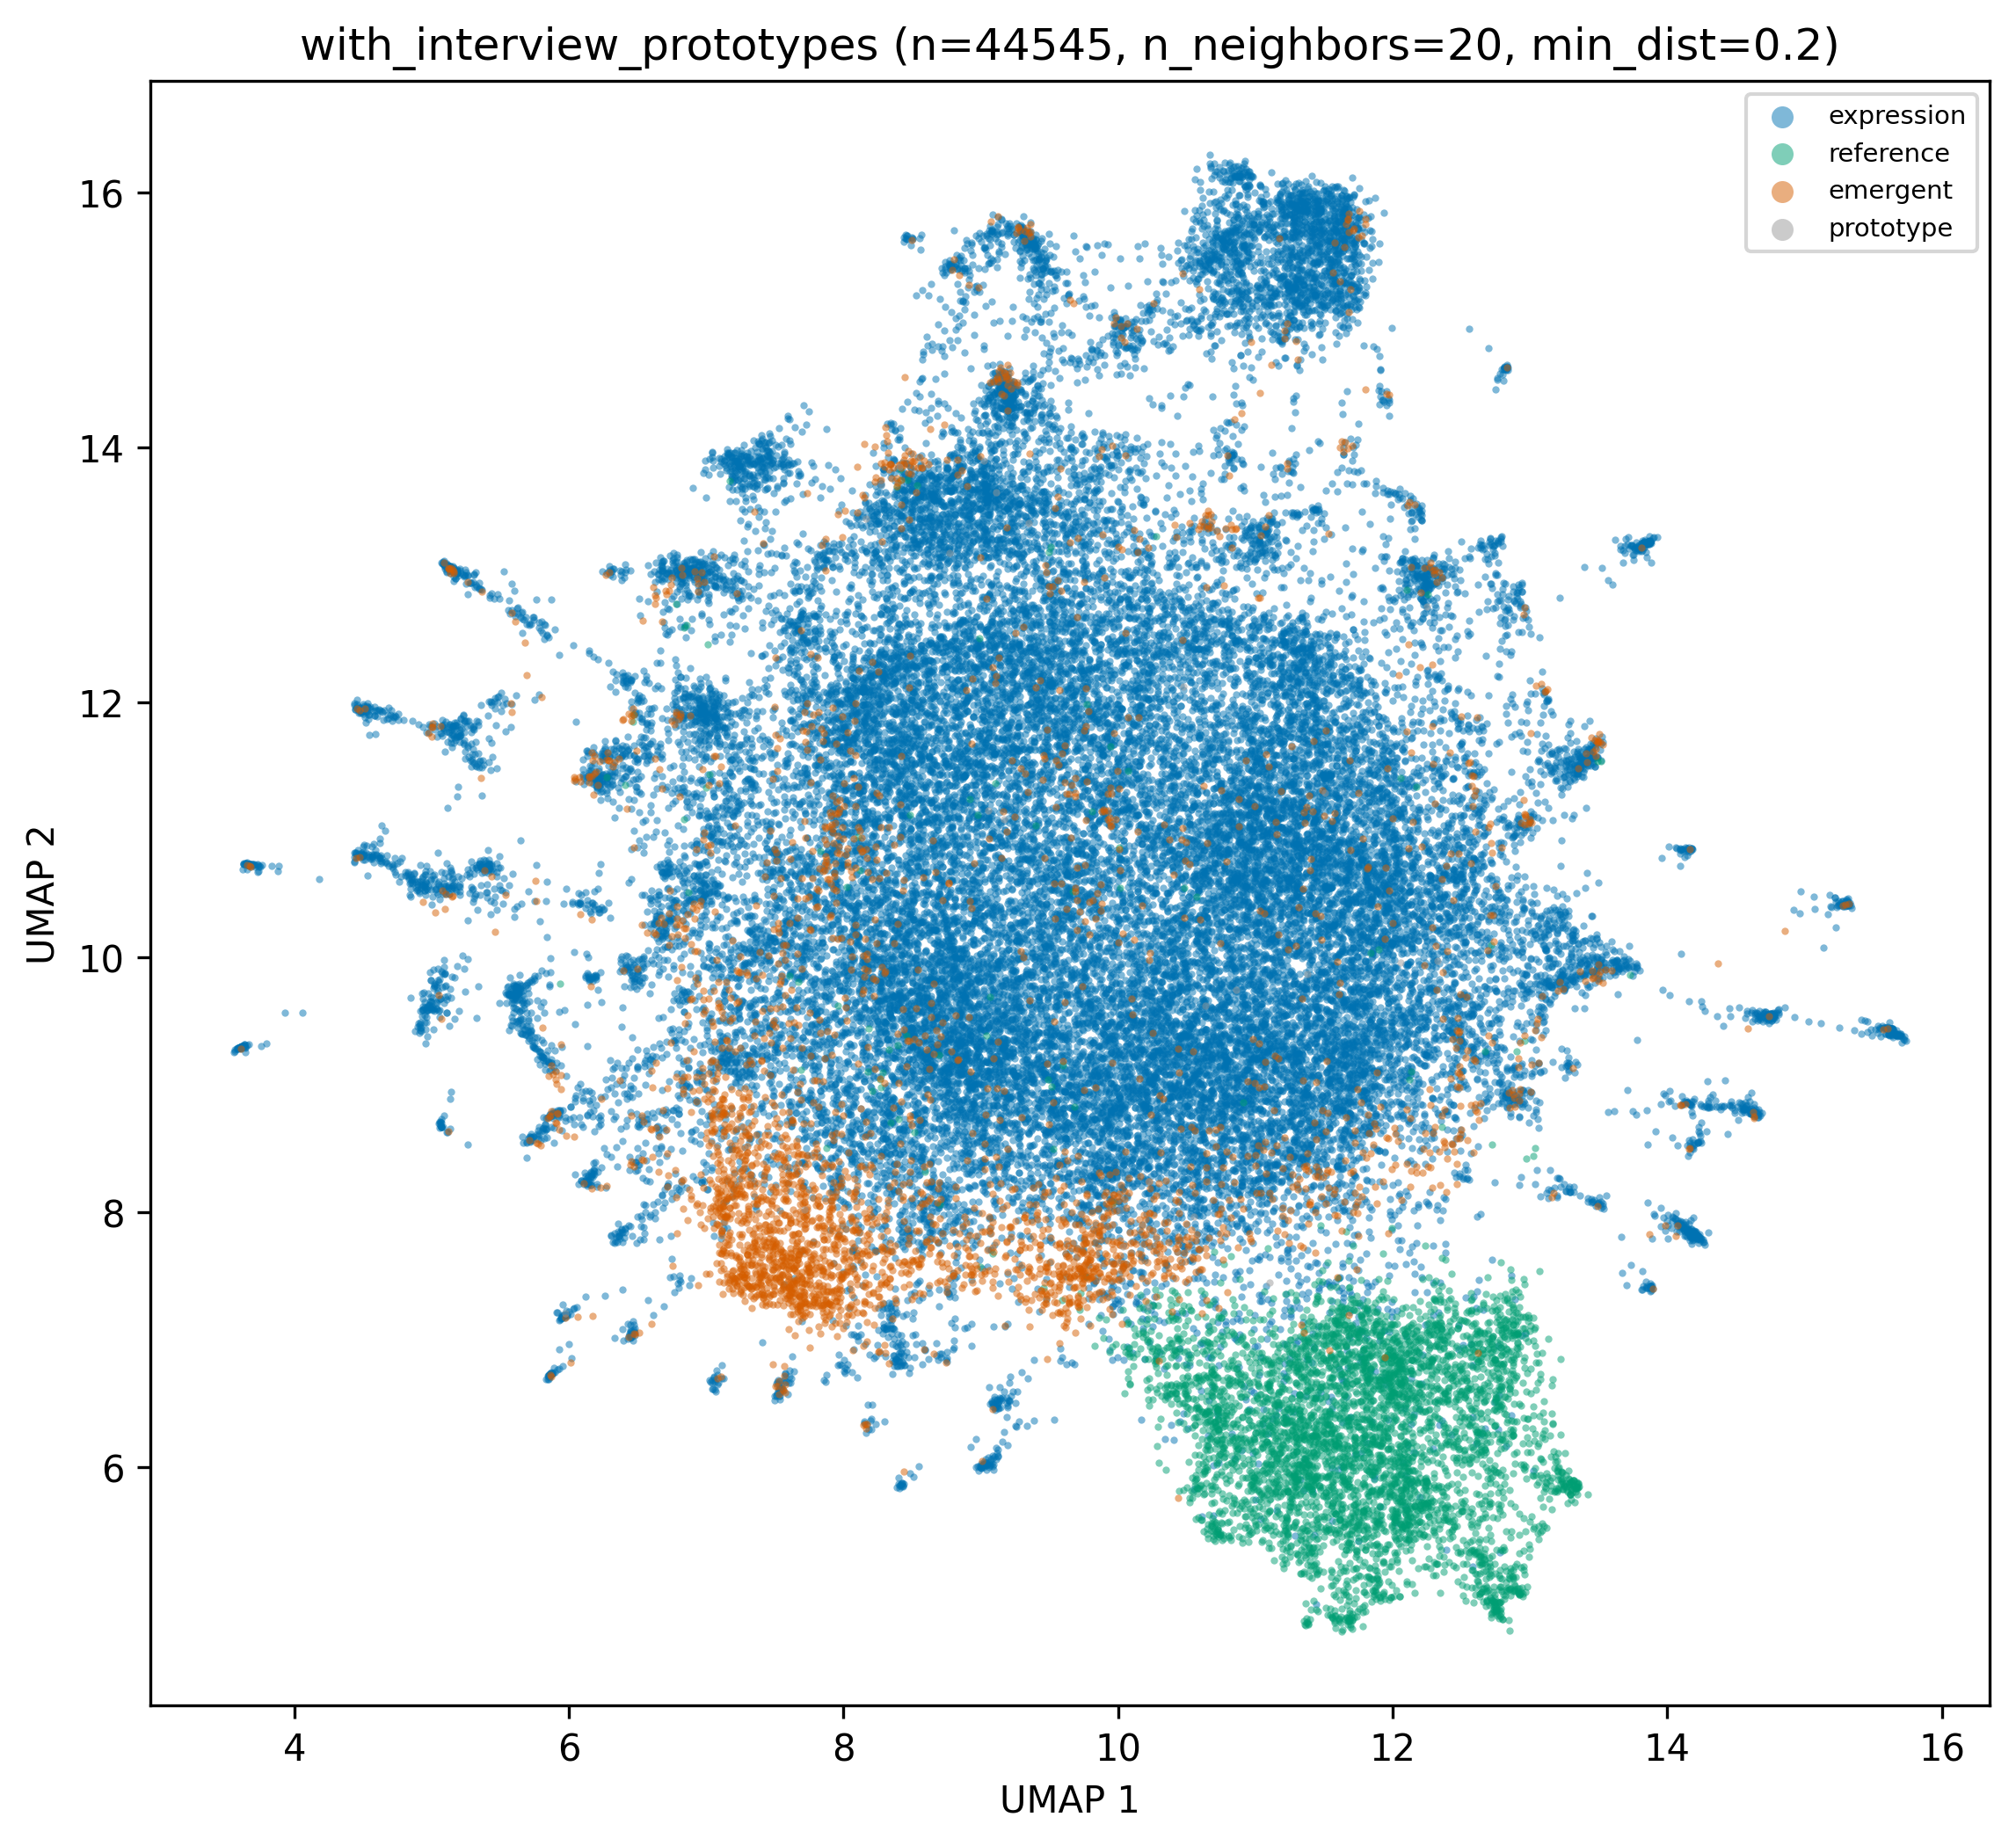
\includegraphics[width=0.85\textwidth]{figures/umap_with_interview_prototypes_by_point_role_n20_d0.2.png}
\caption{Whole-space UMAP with the 25 resolved interview-prototype
points overlaid (point role distinguishes them from ordinary expression
points), coloured by point role.}
\end{figure}

\subsection{Emergent entities: what named things does the corpus actually talk about?}
\jargon{Module: \texttt{analyze\_emergent\_entities}}

This module looks at the 3,251 emergent entities (Stage~4) and asks a
simple provenance question for each one: \emph{which} of the three
corpora mentions it?

\begin{table}[h!]
\centering
\begin{tabular}{lr}
\toprule
Provenance category & Number of entities \\
\midrule
literature\_only & 3{,}111 \\
shared\_2\_corpora & 81 \\
miviludes\_only & 48 \\
shared\_all\_3 & 9 \\
interviews\_only & 2 \\
\bottomrule
\end{tabular}
\caption{Which corpora mention each emergent entity.}
\end{table}

\begin{figure}[h!]
\centering
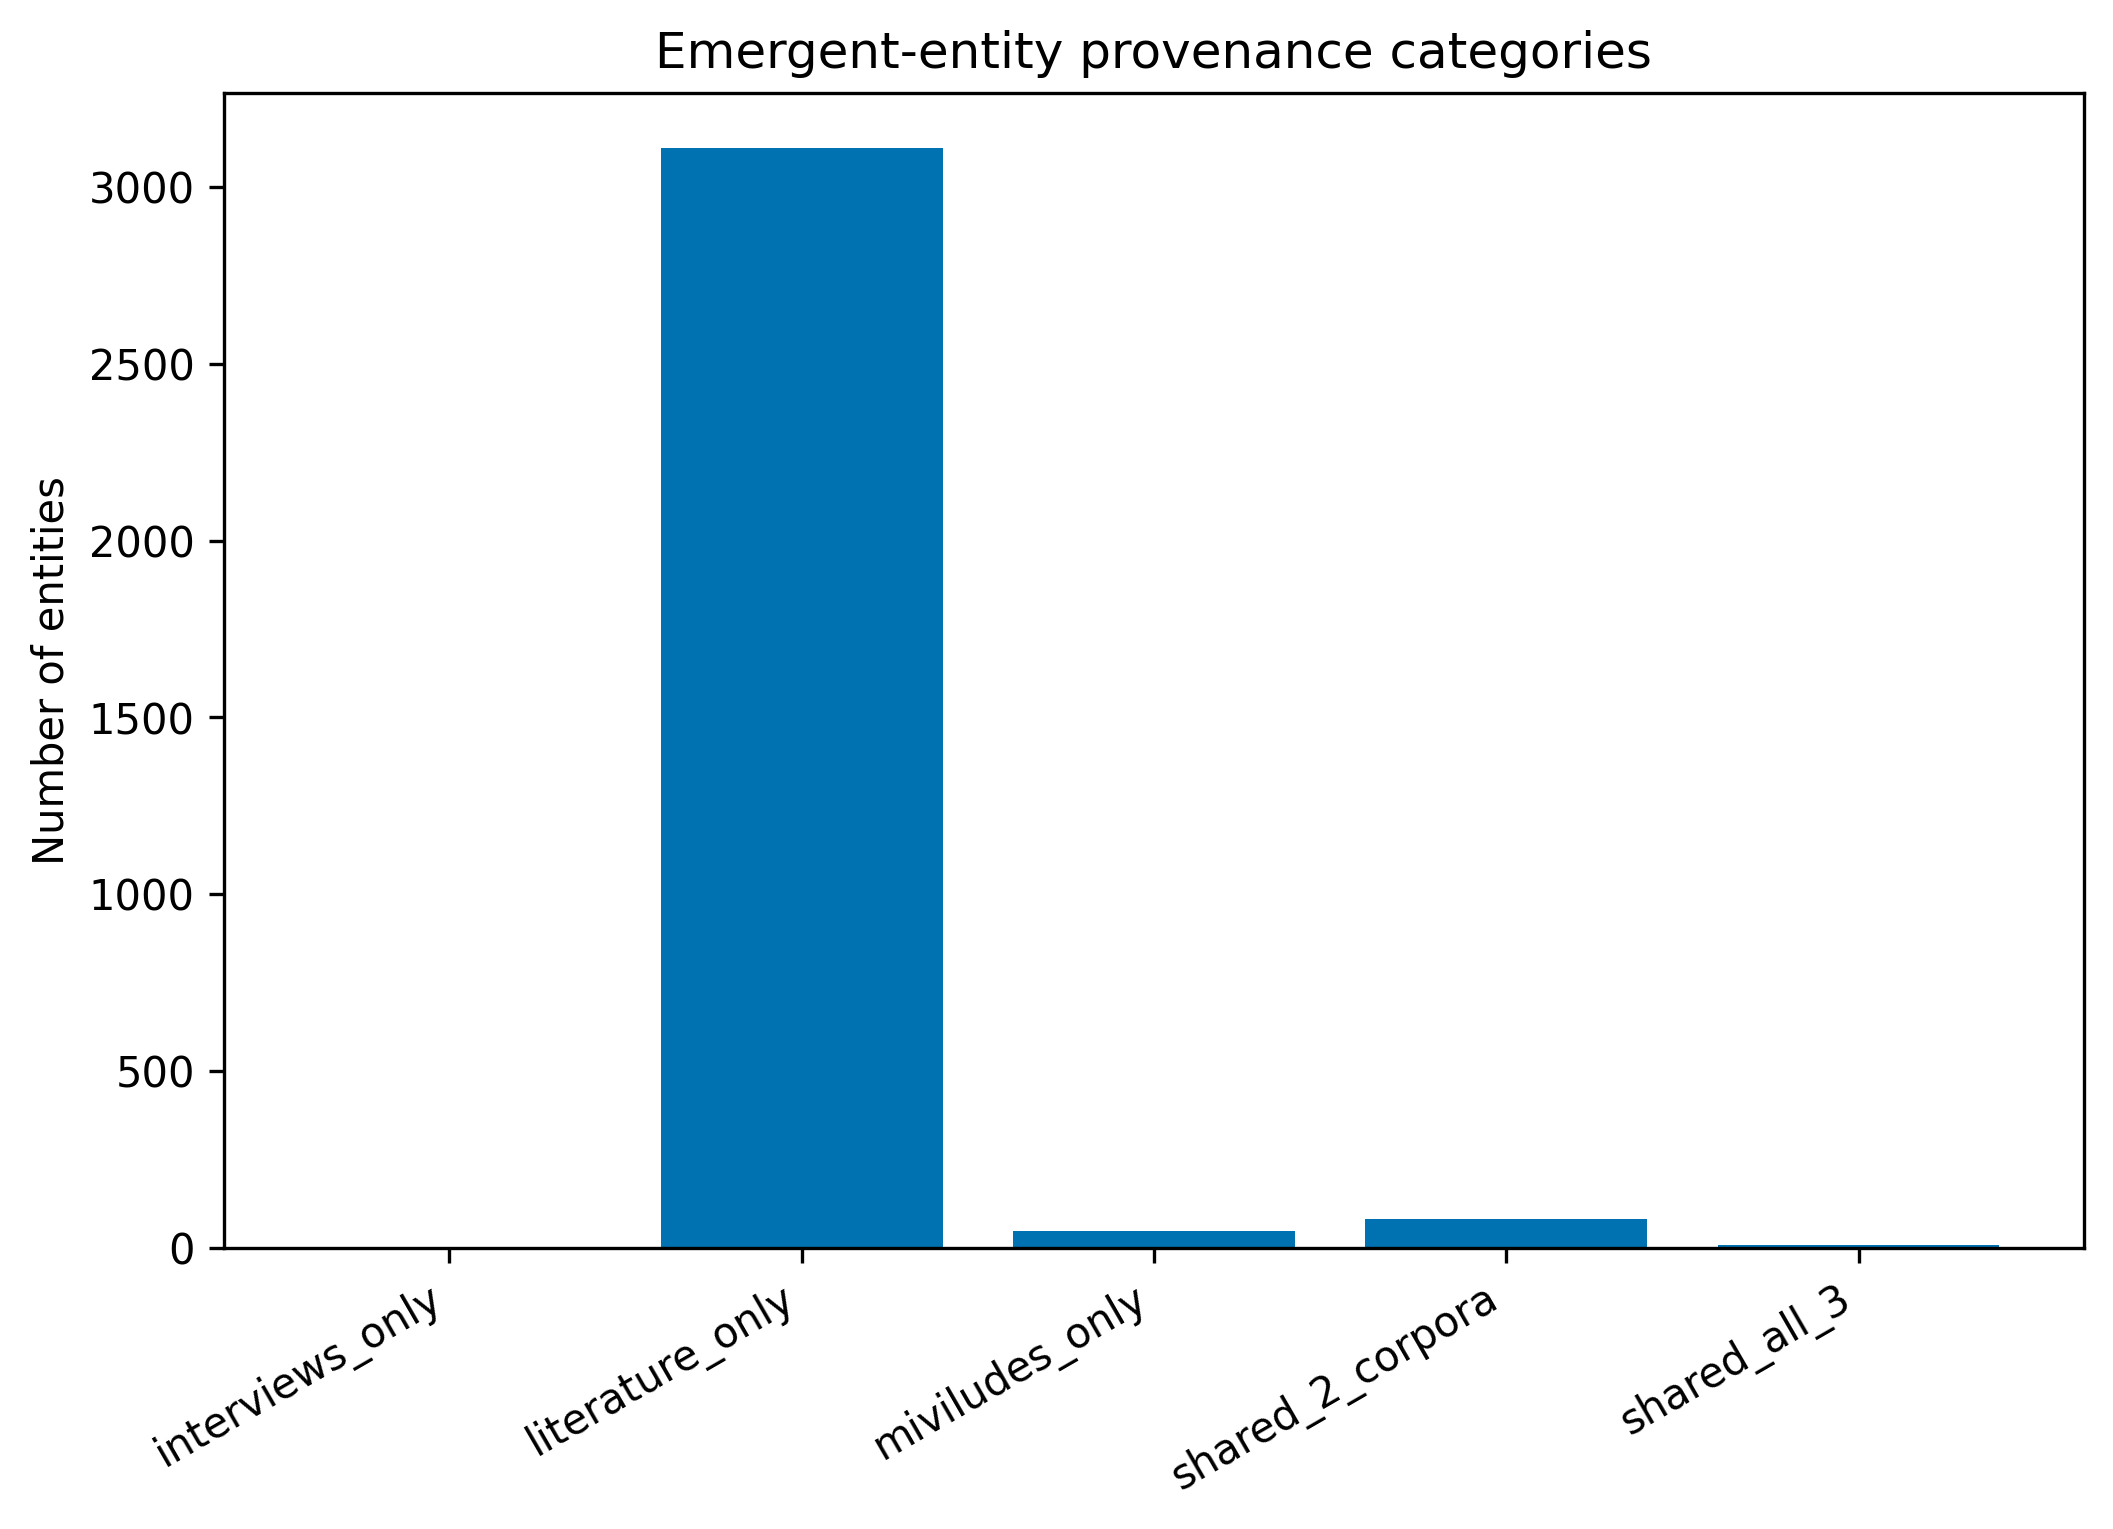
\includegraphics[width=0.7\textwidth]{figures/entity_provenance_categories.png}
\caption{Emergent entities grouped by which corpus/corpora mention
them.}
\end{figure}

In plain terms: the overwhelming majority of named entities (3,111 of
3,251, about 96\%) are mentioned only in the literature -- unsurprising
given literature contributes 97\% of all expression points to begin
with, and a direct consequence of corpus size rather than, by itself,
evidence about what different sources "really" focus on. Only 9
entities are mentioned across all three corpora at once, and just 2 are
mentioned exclusively by the interviews and nowhere else. This module
deliberately does \textbf{not} classify any entity as "genuinely a cult"
versus "mainstream" or apply any other normative label -- it reports
who talks about what, not who is right.

\subsection{Focused projections: readable, curated pictures}
\jargon{Module: \texttt{generate\_focused\_projections}}

The whole-space UMAP pictures shown above are useful for a general
sense of shape, but with over 44,000 points they are too dense to read
any one specific comparison off of directly. This module instead builds
small, curated point-sets around a specific question -- e.g.\ "just the
neighbourhood around one MIVILUDES criterion," "just the interview
prototypes against everything else," "just the emergent-entity
region" -- and projects each one on its own, both via a fresh UMAP fit
and via the same fixed linear PCA basis used everywhere else (so PCA
figures stay comparable to each other specifically). 22 such focused
populations were generated this run, ranging from 46 points (a single
criterion's neighbourhood) up to several thousand (the three big
reference-vocabulary comparisons). Every rendered figure notes how many
points were actually fit versus how many were only overlaid afterward
(e.g.\ corpus centroids, added to the picture after the projection was
already computed, never part of the fit itself) -- see the run's
\texttt{generate\_focused\_projections/config.json} for the full list of
populations and their exact sizes.

% ============================================================
\section{Honesty notes -- what these numbers do not show}
% ============================================================

This section collects, in one place, the caveats already scattered
through the sections above, since they matter for how any of this gets
written up.

\begin{itemize}[leftmargin=1.4em]
  \item \textbf{Corpus imbalance.} Literature is about 97\% of all
  expression points. Any unweighted statistic over the pooled space is
  dominated by literature's own vocabulary and register unless
  explicitly corrected for (as the equal-$n$ cluster-structure numbers
  above are).
  \item \textbf{MIVILUDES is two documents.} Treat MIVILUDES's results
  as one influential operational framework, not a representative sample
  of French state framing in general.
  \item \textbf{The interview sample is a convenience sample.}
  Recruited through the researcher's own network -- exploratory
  prototype evidence, not a representative survey of lay usage.
  \item \textbf{\texttt{response\_rank} is not usable as a
  "first thing they thought of" signal} (Section~\ref{sec:results},
  first subsection) -- only the manually-reviewed initial-exemplar
  layer should be used for interview-side "first impression" claims.
  \item \textbf{Equal-size-controlled comparisons control for pool size
  only.} They are not evidence that the three reference vocabularies
  are otherwise interchangeable -- they still differ in source,
  curation method, and coverage.
  \item \textbf{2-D pictures (UMAP, PCA slices) are a reading aid, not
  evidence.} The actual distance and similarity numbers come from the
  full 394-dimensional space; a 2-D projection can visually compress or
  distort real structure.
  \item \textbf{Three language representations of the MIVILUDES criteria
  are kept separate on purpose} and never averaged together, since they
  answer a "does this hold regardless of language" question rather than
  a "what is the true number" question.
\end{itemize}

% ============================================================
\section{Using this document to write the Results chapter}
% ============================================================

Everything above is deliberately descriptive: what was measured, what
came out, and what it does and does not show. It does not yet answer the
thesis's actual question -- whether the three sources converge on
recurring criteria, whether "cult" fragments into genuinely different
things across academic, institutional, and everyday discourse, or what
kind of category (religious group, social relation, form of authority,
risk category, \ldots) each source implicitly treats it as. That
interpretive step is the point of the Results chapter itself, and is
intentionally left undone here.

Concretely, as raw material for that chapter, this document supplies:
a plain-language glossary that can be trimmed down and folded into the
Methods or Results chapter as needed; the actual current numbers for
global structure, cluster structure, criterion neighbours, interview
exemplars, and emergent entities; a curated set of figures (the ones
embedded here, plus roughly 140 more per-criterion and per-population
figures in \texttt{processed/analysis/20260907-002832/generate\_figures/}
for anything not covered by the ones shown above); and an explicit list
of what these numbers do not license concluding, so that whatever gets
written next stays as epistemically careful as the toolkit's own draft
report already is.

\end{document}
